%% ##############################################################################################
%% Plantilla estándar (en el caso de que exista algo parecido a un estándar) para el documento de tesis para la maestría en ciencias computacionales del INAOEP.
%% Fecha última modificación: 23 de agosto de 2010
%% Editada por: R. Omar Chávez G.
%% Nota: Cualquier mejora o modificación favor de comentarla y distribuirla.
%% ----------------------------------------------------------------------------------------------
%% Registro de modificaciones
%% 
%% ##############################################################################################

\documentclass[12pt,letterpaper,spanish]{book}

% para emcabezados y pies de página
\usepackage{fancyhdr}

% para usar de manera natural los acentos, tildes y así -- además del respectivo diccionario de español 
\usepackage[utf8]{inputenc} 
\usepackage[spanish,activeacute]{babel}
\usepackage{amsmath}
\usepackage{amssymb} 

% para tablas que se pasan de lanza, digo, de largas
\usepackage{longtable} 

% para incluir los apéndices
\usepackage{appendix}

% para incluir gráficas y subgráficas dentro de las gráficas etc., etc.
\usepackage{graphicx}
%\usepackage{subfigure}
\usepackage{wrapfig}
\usepackage{caption}
\usepackage{subcaption}

% para definir algunos márgenes personalizados
\usepackage{anysize}
\marginsize{1.5in}{1in}{1in}{1in}
\usepackage[nottoc]{tocbibind}
\usepackage{setspace}

% para tablas con celdas compartidas
\usepackage{multirow}
\usepackage{fancybox}

% para incluir colores en texto o en celdas de las tablas
\usepackage{color}
\usepackage{colortbl}
\usepackage[table,xcdraw]{xcolor}

% para el estilo natbib de bibliografías (sino lo usan no va)
\usepackage{natbib}

\usepackage{titlesec}

% para incluir páginas de un archivo pdf
\usepackage{pdfpages}

%para incluir archivos SVG
\usepackage{svg}


%##############################################################################
% para renombrar algunos títulos
\renewcommand{\appendixname}{Apéndices}
\renewcommand{\appendixtocname}{Apéndices}
\renewcommand{\appendixpagename}{Apéndices}

%##############################################################################
% incluimos información personalizada para algunos valores de la plantilla
\newcommand{\tstamp}{\small [\thepage]}
\newcommand{\Escuela}{\scshape \scriptsize Coordinaci\'{o}n de Ciencias Computacionales}
\newcommand{\Uni}{\scshape \scriptsize Instituto Nacional de Astrof\'{i}sica, \'{O}ptica y Electr\'{o}nica}
\newcommand{\TEMA}{\scshape \scriptsize Aumento de datos para tareas relacionadas al perfilado de autor.}


%##############################################################################
% redefinimos los espacios para las figuras

\newcommand{\figura}[5]{
  \begin{figure}[#5]
  \begin{center}
  \includegraphics[#2]{#1}
  \caption[#3]{#3}
  \label{#4}
  \end{center}
  \end{figure}
}
%##############################################################################
% redefinimos los espacios para las tablas
\newenvironment{tabla}[2]{
  \begin{table}[#2]
  \begin{center}
  \caption[#1]{#1}
}{
  \end{center}
  \end{table}
}

%##############################################################################
% renombramos algunas constantes para entornos matemáticos
\def\sen{{\rm sen \ }}
\def\cos{{\rm cos \ }}

\def\a{\mathbf a}
\def\b{\mathbf b}
\def\c{\mathbf c}
\def\d{\mathbf d}
\def\e{\mathbf e}
\def\ex{\mathrm e}
\def\f{\mathbf f}
\def\g{\mathbf g}
\def\h{\mathbf h}
\def\k{\mathbf k}
\def\n{\mathbf n}
\def\m{\mathbf m}
\def\p{\mathbf p}
\def\q{\mathbf q}
\def\P{\mathbf P}
\def\R{\mathbf R}
\def\T{\mathbf T}
\def\L{\mathbf L}
\def\r{\mathbf r}
\def\u{\mathbf u}
\def\v{\mathbf v}
\def\w{\mathbf w}
\def\x{\mathbf x}
\def\y{\mathbf y}
\def\z{\mathbf z}
\def\sen{{\rm sen \ }}

%################################################################################
% rebombramos las etiquetas para retuilizar la información antes ingresada
\renewcommand{\labelenumi}{\textbf{\theenumi}.-}
\renewcommand{\labelenumii}{\textbf{\theenumi}.-}
\renewcommand{\labelenumiii}{\textbf{\theenumi}.-}
\renewcommand{\labelenumiv}{\textbf{\theenumi}.-}



%#################################################################################
% especificamos casos extraodinarios para la división de palabras
\hyphenation{es-pe-cia-li-dad} \hyphenation{ob-te-ner}
\hyphenation{des-ple-gar}
\hyphenation{original}
\hyphenation{geo-gra-fi-ca} \hyphenation{do-cu-men-to}
\hyphenation{do-cu-men-tos} 
\hyphenation{e-va-lua-da}\hyphenation{pro-pues-ta}
\hyphenation{tu-ris-mo}\hyphenation{pro-pues-to}
\hyphenation{ma-yo-res}\hyphenation{des-cri-be}
\hyphenation{re-le-van-cia}\hyphenation{pro-ble-ma}
\hyphenation{ma-ne-ra}\hyphenation{co-rres-pon-de}
\hyphenation{pro-pues-to}\hyphenation{re-tro-a-li-men-ta-cion}
\hyphenation{si-mi-li-tud}\hyphenation{tradicional}\hyphenation{ordenamiento}
\hyphenation{pu-bli-ca-cio-nes}\hyphenation{a-tri-bu-tos}
\hyphenation{re-cu-pe-rar}\hyphenation{re-cu-pe-ra-das}

% espaciado : 1 y 1/2
\onehalfspacing

% establecemos la enumeración para las equaciones y figuras
\numberwithin{equation}{section}
\renewcommand{\thefigure}{\thechapter.\arabic{figure}}

\setlength{\arrayrulewidth}{1pt}
\setlength{\doublerulesep}{0mm}

\sloppy
\frenchspacing

% redefinimos el comando para incrustar dos páginas vacías
\newcommand{\clearemptydoublepage}{\newpage{\pagestyle{empty}\cleardoublepage}}


%#################################################################################
% inicio del documento

\begin{document}

% incluimos el pdf con la portada (sólo la página 1) (la azul fea) como primera página de este documento
% nota: debes modificar y compilar de manera separada el archivo portada.tex, luego compilar este documento para que incluya la versión modificada del PDF (portada.pdf)

\includepdf[pages={1}]{portada.pdf}
\clearemptydoublepage

% incluimos el .tex que tiene la información para la contraportada (puede llamarse como desees, pero recuerda poner el nombre sin extensión)
\begin{titlepage}
\begin{center}
{\Large \scshape \bf Aumento de datos para tareas relacionadas al perfilado de autor}
%{\Large \scshape \bf Ordenamiento de Imágenes Recuperadas Utilizando una Combinación de Características Visuales y Textuales}\\
%{\bf \emph{Coordinaci\'{o}n de cs. Computacionales}}
\end{center}

\vspace*{\fill}
\begin{center}
{Tesis de Maestría}
\end{center}

\vspace*{\fill}
\begin{center}
{\large \scshape Por:}
\end{center}

\begin{center}
{\Large \bf Víctor Jiménez Villar}
\end{center}

\vspace*{\fill}
\begin{center}
{\scshape Asesor:}\\
{\bf \scshape Dr. Luis Villaseñor Pineda} 
%\\
%{\bf \scshape Dr. Luis Enrique Sucar Succar}
\end{center}

\vspace*{\fill}
\begin{center}
{Instituto Nacional de Astrof\'{i}sica \'{O}ptica y Electr\'{o}nica}\\
{Coordinaci\'{o}n de Ciencias Computacionales}
\end{center}

\vspace*{\fill}
\begin{center}
\begin{tabular}{cc}
\multicolumn{1}{p{2.5in}}{\centering \scriptsize
\textsc{Tonantzintla, Puebla.}}&
\multicolumn{1}{p{2.5in}}{\centering \scriptsize \textsc{Agosto 2020}}\\
\end{tabular}
\end{center}
\end{titlepage}

\clearemptydoublepage


\frontmatter
\pagestyle{fancyplain}



%###############################################################################33
% redefinimos los márgenes para el documento
\setlength{\topmargin}{0.0cm}
\setlength{\headsep}{0.5cm}
\setlength{\headheight}{0.5cm}

\setlength{\marginparsep}{0mm}
\setlength{\marginparwidth}{0cm}

\setlength{\footskip}{1.5cm}

  \setlength\paperheight {11in}
  \setlength\paperwidth  {8.5in}

  \setlength{\textwidth}{6in}
  \setlength{\textheight}{8.5in}

  \setlength{\marginparwidth}{0cm}
  \setlength{\voffset}{0.0in}
  \setlength{\hoffset}{0.0in}

  \setlength{\evensidemargin}{0in} % margen par
  \setlength{\oddsidemargin}{0.32in}  % margen impar
 % \setlength{\oddsidemargin}{0in}  % margen impar



%###################################################################################
% especificamos el nombre en español para cada sección estándar de la tesis
%\def\contentsname{\'{I}ndice General}
\def\contentsname{Tabla de Contenido}
\def\listfigurename{Lista de Figuras}
\def\listtablename{Lista de Tablas}
\def\bibname{Bibliografía}
\def\indexname{\'{I}ndice Alfabético}
\def\figurename{\bf \scriptsize Figura}
\def\tablename{\bf \scriptsize Tabla}
\def\partname{Parte}
\def\chaptername{Cap\'{i}tulo~\thechapter}
\def\appendixname{Ap\'{e}ndice}
\def\abstractname{Resumen}


% presentación de título y capítulo
\renewcommand{\chaptermark}[1]{\markboth{#1}{}}
% número y título de sección
\renewcommand{\sectionmark}[1]{\markright{\thesection~~ #1}}




\lhead[\fancyplain{}{\small \thepage}]{\fancyplain{}{\scshape
\scriptsize \rightmark}} %\rightmark = información sobre el capítulo

\rhead[\fancyplain{}{\scshape \scriptsize
\leftmark}]{\fancyplain{}{\small \thepage}} %\leftmark = información sobre la sección

\lfoot[\fancyplain{}{\Escuela}]{\fancyplain{}{}}
\cfoot[\fancyplain{\tstamp}{}]{\fancyplain{\tstamp}{\TEMA}}
\rfoot[\fancyplain{}{\Uni}]{\fancyplain{}{}}

\renewcommand{\headrulewidth}{0.4pt}
\renewcommand{\footrulewidth}{\headrulewidth}

% cambiar el formato para los títulos
\newcommand{\bigrule}{\titlerule[0.5mm]}

\titleformat{\chapter}[display]
{\bfseries \Huge } {
 \titlerule
 \filleft\Large\chaptertitlename
 }
{0mm} {\filleft}
 [\vspace{0.5mm}\bigrule]


% incluimos los .tex de cada uno de las secciones previas al verdadero documento (recuerda: sólo debe ir el nombre del .tex)
% los puntos .tex van sin preámbulo, es decir que sólo va el texto correspondiente y las instrucciones para definir título, secciones, subsecciones, tablas, etc.

\chapter{Agradecimientos}

Esta investigación fue realizada gracias al apoyo otorgado por el Consejo Nacional de Ciencia y Tecnología (CONACYT), a través de la beca No. 718947. 

Al INAOE, por brindarme la oportunidad de continuar con mi formación profesional. Gracias a todos los investigadores de la coordinación de Ciencias Computacionales que con su amabilidad y paciencia logre comprender los fundamentos teóricos para realizar este trabajo. 

A mi asesor, Luis Villaseñor Pineda, por dirigir esta investigación de la mejor forma posible, siempre dándome sugerencias sobre cómo mejorar mi trabajo.

Al doctor Manuel Montes y Gómez el cual sin ser mi asesor siempre se mantuvo al pendiente de mis avances.

Al doctor Francisco Martínes Trinidad, por enseñarme los fundamentos teóricos en aprendizaje computacional, manteniendo una crítica objetiva sobre mi trabajo.

Al doctor Aurelio López López, por sus clases en procesamiento de lenguaje natural y sus aportes para corregir la claridad de este documento.

A Luz Maria Romero Cirne, por ayudarme a corregir los errores ortográficos en este documento.

A mis familiares y amigos por apoyarme en esta aventura.




\chapter{Dedicatoria}

A mi familia y amigos, por motivarme cada día superar mis límites. 


\include{resumen}

% por si quieres incuir hasta un tercer nivel en la tabal de contenidos
%\setcounter{tocdepth}{3}

% creamos la tabla de contenidos y las listas de figuras y tablas
\tableofcontents
\listoffigures 
\listoftables

\mainmatter
\renewcommand{\chaptermark}[1]{\markboth{\thechapter.~~#1}{}}

%########################################################################################
% ahora si incluimos cada uno  de los .tex correspondientes a los capítulos de la tesis. Es más claro dividir los capítulos en .tex aunque puedes poner tooodo el texto aquí.
% los puntos .tex van sin preámbulo, es decir que sólo va el texto correspondiente y las instrucciones para definir título, secciones, subsecciones, tablas, etc.
\chapter{Introducción}

Imagina que se te ha dado un texto de un autor anónimo, y deseas saber tanto como sea posible del autor (género, ocupación, personalidad etc.), sólo analizando el texto dado. Es sorprendente, pero el texto refleja parte de la personalidad del autor. Así que, observando el texto al determinar su estilo y contenido, es posible inferir información sobre el autor. A esta tarea se le conoce como \textit{perfilado de autor} y está fundada en estudios dentro de la comunidad sociolingüística, demostrando que las palabras utilizadas en la vida diaria pueden revelar importantes aspectos sociales y psicológicos. Gracias a los avances en computación, el análisis de textos permite a los investigadores obtener características de lo que las personas dicen y también de las particularidades en sus estilos lingüísticos \citep{Pennebaker2002}. 

El interés en esta tarea ha crecido gracias al constante flujo de información compartida a través de redes sociales (por ejemplo, Twitter \footnote{www.twitter.com}, Facebook\footnote{www.facebook.com} y Reddit \footnote{www.reddit.com}) y sus aplicaciones varían desde mercadotecnia hasta seguridad nacional. 
Existen numerosas razones del por qué nos interesa conocer datos relevantes de los usuarios de redes sociales. Por ejemplo, a las empresas les interesaría conocer a qué tipo de usuarios les gusta o no su producto o servicio, con la intención de dirigir una mejor campaña de publicidad \citep{ikeda2013twitter}. Además, en un contexto de seguridad informática, a la policía cibernética le gustaría conocer el perfil de las personas que envían mensajes amenazantes o de acoso sexual \citep{bogdanova2012impact}.

Claro está que la tarea no es simple y debido al lenguaje informal de redes sociales y poco estandarizado hace que esta tarea sea aún más desafiante, por ejemplo: errores gramaticales, abreviaturas, anglicismos, emoticonos o incluso texto generado por cuentas automáticas. Una de las conferencias más destacadas en perfilado de autor ha sido el PAN@CLEF\footnote{www.pan.webis.de} (una serie de eventos científicos y tareas compartidas en el análisis forense digital y estilométrico); desde el año 2013 al actual se han estudiado diversos enfoques del perfilado de autor desde una perspectiva multi-idioma (inglés y español principalmente) entre las cuales destacan: identificación de edad y género \citep{Rangel2013b}, identificación de personalidad, variación de lenguaje y dimensión de género \citep{Stammatatos2015}. 

Un tema de particular importancia es el perfilado de características de comportamiento \citep{kumar2018aggression} y condiciones médicas \citep{de2013predicting}; estas tareas se han desarrollado en subcampos y con sus propias conferencias. Por ejemplo, la conferencia eRisk \citep{Losada2018}, está orientada al perfilado del autor en búsqueda de evidencia de trastornos como la depresión o la anorexia. El perfilado automático de depresión y anorexia consiste en recopilar una serie de textos de diferentes autores, con el objetivo de extraer información útil para construir modelos estadísticos, que permitan predecir signos de depresión y anorexia. La hipótesis inicial es que los cambios en el lenguaje de un autor, empleado para interactuar y expresarse diariamente, contiene patrones que pueden indicar este tipo de desórdenes mentales \cite{de2013predicting}.



\section{Planteamiento del problema}

Para resolver las tareas de perfilado de autor, la mayoría de los trabajos existentes se han enfocado en utilizar algoritmos de aprendizaje computacional, en combinación con diferentes técnicas para extraer características: conteo de palabras \citep{Laserna2014}, identificación de frases personales \citep{Ortega-Mendoza2018}, análisis de emociones \citep{Aragon2019} entre otras técnicas. La obtención de dichas características requiere un análisis riguroso y en muchos casos es necesaria la intervención de expertos en el tema. No obstante, existen técnicas de aprendizaje computacional más complejas como las redes neuronales, en donde la extracción de características se realiza de forma automática mediante una serie de abstracciones.

La principal motivación para el uso de redes neuronales en perfilado de autor, es debido al increíble éxito del aprendizaje profundo en tareas complejas para el entendimiento del lenguaje: parafraseo, traducción automática, analogía, implicación textual, similitud semántica, etc. En el conjunto de datos GLUE \citep{wang2018glue}, los modelos de aprendizaje profundo han superado la puntuación humana, Christopher D. Manning (director del laboratorio de inteligencia artificial de la universidad de Stanford), menciona que desde el año 2015 se produjo un tsunami del aprendizaje profundo en el área de procesamiento de lenguaje natural, debido a la gran cantidad de artículos en conferencias de NLP utilizando aprendizaje profundo \citep{Manning2015}.

De acuerdo al estado del arte, en la última conferencia del PAN@CLEF los equipos con mejores resultados utilizaron técnicas tradicionales de aprendizaje como lo son máquinas de soporte vectorial SVM, en combinación con n-gramas de caracteres. Así también, en las tareas del eRisk el mejor sistema se construyó extrayendo características en combinación con un ensamble de bolsas de palabras (BOW por sus siglas en inglés) y diferentes clasificadores. Lo que se ha podido observar en los diferentes reportes de estas conferencias es que los modelos de aprendizaje basados en redes neuronales no han tenido el éxito esperado. 

Uno de los principales problemas dentro del campo de aprendizaje automático es que el éxito de éste depende de la cantidad de datos etiquetados con que se cuente y se hace más notable cuando se utilizan modelos de aprendizaje profundo, el etiquetado manual de datos consume mucho tiempo y es costoso, además se podría incurrir en problemas legales debido al uso de datos personales, como es el caso en las tareas de perfilado de autor. Los estudios actuales tratan con un número pequeño de autores conocidos, en donde el etiquetado manual puede ser aplicado, pero considerando las dimensiones de los datos en redes sociales se convierte en una tarea costosa y difícil.

Uno de los problemas conocidos en la clasificación de textos es el sobreajuste de los modelos de aprendizaje, el cual se genera en la etapa de entrenamiento debido a que el modelo memoriza los pocos documentos de entrenamiento. Por lo tanto, ante esta situación es deseable tener una una amplia diversidad en los textos, es decir tener frases que signifiquen los mismo pero escritas de forma diferente; para esto se han propuesto diferentes técnicas como el aumento de datos o agregar ruido aleatorio a los ejemplos originales.

Observando las limitantes anteriores este trabajo presenta un estudio incrementando el conjunto de datos de entrenamiento, observando el efecto al agregar documentos nuevos. Para ello, se crean nuevos documentos respetando su estructura, y se agregan al conjunto de entrenamiento original. Este estudio analiza el efecto que tiene este incremento en los algoritmos de redes neuronales tradicionales en tareas relacionadas al perfilado de autor. 

Algunas de las principales preguntas a contestar en esta investigación son:

\begin{enumerate}
    \item {¿Cómo conservar el estilo y contenido para el aumento de datos en perfilado de autor?}
    \item ¿En qué tipo de arquitecturas basadas en redes neuronales tiene mayor impacto el aumento de datos?
    \item ¿Se puede mejorar el perfilado de usuarios que sufren depresión y anorexia mediante el aumento de datos?
\end{enumerate}


\section{Objetivo general}

Proponer un método de aumento de datos, considerando estilo y contenido del texto, para mejorar la predicción de los modelos de aprendizaje profundo en las tareas de perfilado de autor.


\section{Objetivos específicos}
\begin{enumerate}
    \item Diseñar diferentes estrategias de aumento de datos bajo condiciones supervisadas, que permita conservar el estilo y contenido del documento original y a la vez aumentar el vocabulario.
    \item Demostrar el efecto del aumento de datos tanto en modelos de redes neuronales como en modelos de aprendizaje supervisado tradicionales.
    \item Evaluar y analizar los métodos propuestos para abordar el perfilado de depresión y anorexia en redes sociales.
 
\end{enumerate}

\section{Organización de la tesis}

Esta tesis está organizada de la siguiente forma: 

%%Capitulo 1- Pendientes 
%% Refinar preguntas de investigación
%% Defninir hipotesis

\begin{itemize}
\item Capítulo 2: \textbf{Marco teórico}. Presenta una rápida introducción a la clasificación de textos con aprendizaje automático, además de mencionar las principales métricas de evaluación utilizadas en este trabajo. Los conceptos descritos son fundamentales para comprender la solución propuesta.


\item Capítulo 3: \textbf{Trabajo relacionado}. Describe el estado del arte en perfilado de autor y aumento de datos para clasificación de textos, su principal objetivo es conocer como se ha abordado el problema y analizar las ventajas y desventajas de los métodos existentes.

%%%Cuadro comparativo de ventajas y desventajas de los diferentes metodos


\item Capítulo 4: \textbf{Método propuesto}: En este capítulo se describen a detalle los métodos propuestos, su justificación y algunos ejemplos de aumento de datos.

\item Capítulo 5: \textbf{Configuración experimental y resultados}: En este capítulo se describen los conjuntos de datos estudiados y la configuración para los distintos clasificadores empleados, así como los métodos propuestos y los métodos de referencia o de comparación. Se realiza una comparación de los resultados obtenidos con el estado del arte para la detección de depresión y anorexia.

\item Capítulo 6: \textbf{Conclusiones y trabajo futuro:} Por último se exponen las principales contribuciones de este trabajo y formas en que se puede mejorar.

\end{itemize}


\chapter{Marco Teórico}

En este capítulo se describen conceptos relacionados con la tarea de perfilado de autor mediante algoritmos de aprendizaje automático. Se describen las principales representaciones de un texto dado, las características generales de los clasificadores empleados, así como las medidas de evaluación empleadas para medir los resultados de los diferentes modelos. Además se presenta una introducción de las  tareas de procesamiento de lenguaje natural utilizadas en el método propuesto: etiquetado de partes de la oración, paráfrasis y resolución de analogías.

\section{Clasificación de textos}

En años recientes, ha habido un crecimiento exponencial en el número de textos disponibles en Internet, a tal grado que es imposible procesarlos manualmente, de ahí la importancia de su procesamiento automático. Los problemas de clasificación automática de textos han sido ampliamente estudiados en las últimas décadas, especialmente con los avances en procesamiento de lenguaje natural, muchos investigadores están interesados en desarrollar aplicaciones que mejoren los métodos de clasificación de textos. Las tareas exploradas en este trabajo se circunscriben a las tareas de perfilado de autor, donde se desea conocer la categoría (clase o tipo de autores) a la que pertenece un documento dado (historial del usuario).

\subsubsection{Definición}

La clasificación de textos puede ser definida como la tarea de categorizar un grupo de documentos en una o más clases predefinidas de acuerdo con sus temas \citep{Kadhim2019}. Retomando la definición de \citep{Kadhim2019}, se parte con un grupo específico de documentos $D={\begin{Bmatrix} d_1 , ... , d_n \end{Bmatrix}}$, con clases predefinidas $C={\begin{Bmatrix} c_1 , ... , c_m \end{Bmatrix}}$ y un nuevo documento $q$ el cual es generalmente indicado como una consulta, con el objetivo de predecir la clase del documento consultado, la cual puede ser una o más clases pertenecientes a $C$.

De acuerdo con \citep{kowsari2019text}, la clasificación de textos puede describirse en cuatro pasos: extracción de características, reducción de dimensionalidad o selección de características, construcción del modelo de clasificación y evaluación. A continuación, se describen en forma resumida algunos de los puntos más importantes para este trabajo, tomados del análisis de \citep{kowsari2019text}.

\section{Extracción de características}
El preprocesamiento y la extracción de características, son pasos muy importantes en la clasificación de textos, en las siguientes secciones se presentan algunas de las técnicas más empleadas y se mencionan dos métodos de representación de características: la bolsa de palabras y las representaciones distribucionales.

\subsection{Preprocesamiento}
Dependiendo de la tarea de clasificación, algunos elementos pueden desecharse para enfocar nuestra atención en los elementos más informativos. Algunos de estos elementos son: \textit{palabras de paro}, errores gramaticales, signos de puntuación, etc. Además de esto, el texto extraído de redes sociales contiene enlaces del Internet, menciones de usuario, etiquetas (conocidos como hashtags), emoticonos y un vocabulario muy informal (p.e. abreviaturas no convencionales). A continuación, se explican brevemente algunas técnicas empleadas para el limpiado y preprocesamiento de textos.

\begin{enumerate}
\item \textbf{Tokenización}: Es un método de preprocesamiento en el cual se divide una cadena de caracteres en palabras, frases, símbolos y otros elementos dentro del texto, llamados \textit{tokens} \citep{kowsari2019text}. Se pueden utilizar diferentes algoritmos, para este proceso, lo más simple es separar el texto mediante un espacio o carácter común, por ejemplo:

Texto original: \textit{``Los días de verano son calurosos''}.

Los tokens del texto anterior son los siguientes: \{``Los'',  ``días'', ``de'', ``verano'', ``son'', ``calurosos''\}'

\item \textbf{Palabras de paro}: Son palabras con mayor frecuencia en los documentos, y por lo tanto poco útiles para la discriminación entre documentos de diferentes clases. Ejemplos de ellas son: \{``\textit{a}'' ``\textit{the}'', ``\textit{they}'', ``\textit{he}'' , ``\textit{she}'', ...\} (para el idioma inglés). En algunas tareas de clasificación de textos, las palabras de paro no son de importancia y lo más común es removerlas de los documentos. Nothman \citep{nothman2018stop} presenta un análisis de las palabras de paro y su impacto en la clasificación de textos.

\item \textbf{Capitalización}: Los textos contienen diversas formas de capitalización de palabras para formar una oración. Dado que los documentos consisten en muchas oraciones, una capitalización diversa puede ser muy problemática en la clasificación de textos largos. La técnica más común para tratar la capitalización inconsistente es reducir cada palabra a minúsculas \citep{kowsari2019text}.

\item \textbf{Reducción de ruido}: La mayoría de los textos contienen caracteres innecesarios para la clasificación de documentos, como signos de puntuación o caracteres especiales. En tareas como detección de autoría pueden ser útiles, pero en general agregan ruido a los modelos de clasificación de textos.

\item \textbf{Lematización}:  Es el proceso de convertir palabras a su forma base o raíz (e.g., morfema base del significado) \citep{kamath2019deep}. La desventaja es que este método requiere un diccionario y tablas de búsqueda \citep{kamath2019deep}. Uno de los algoritmos más populares es el algoritmo de Porter \citep{porter2001snowball}, el cual hace una lematización por fuerza bruta mediante el truncamiento de las palabras.

\item  \textbf{Otras técnicas}: Adicionalmente a las técnicas descritas, también es posible preprocesar los textos para intentar normalizarlos, con la intención de facilitar al clasificador la identificación de patrones. Algunas de ellas son: la corrección de errores ortográficos, enmascaramiento de textos, etiquetado de partes de la oración, etc.

\end{enumerate}


\subsection{N-Gramas}
Es una técnica para extraer características para representar un texto, los n-gramas son un conjunto de palabras o caracteres que respetan el orden de aparición en el texto; el número $n$ indica la longitud de la secuencia a considerar, lo más común es utilizar valores de $n$ pequeños (uni-gramas, bi-gramas, tri-gramas) \citep{kowsari2019text}. 

\textbf{Ejemplo de bi-gramas}: 

Texto Original: \textit{``Con el tiempo todo pasa''}

Bi-gramas:\{``con el", ``el tiempo", ``tiempo todo", ``todo pasa"\}


\subsection{Bolsa de palabras BoW}
El modelo de bolsa de palabras o BoW (por sus siglas en inglés ``Bag of Words'') es una representación simplificada de un texto. Normalmente, se utiliza un criterio o pesado específico, como lo puede ser la frecuencia de cada palabra, para representar cada texto. Es decir, en el modelo BoW, el conjunto de documentos es representado mediante una matriz de pesos, siendo las columnas palabras únicas del conjunto de datos y las filas representan un documento. Este modelo es muy simple, donde no es posible capturar el orden secuencial de las palabras -como en una oración o un documento-, con lo que las relaciones semánticas entre las palabras se pierden. Sin embargo, en este modelo las palabras capturan el contenido de un documento y esta representación puede ser utilizada para determinar el tema principal del documento \citep{kowsari2019text}.


\subsubsection{Pesado de palabras} La forma más básica de pesado de características es mediante el pesado \textit{TF} (\textit{term frequency} por sus siglas en inglés), el cual consiste en contar el número de ocurrencias de cada término $t$ en el documento $d$. Los métodos basados en \textit{TF} generalmente consisten en representar la frecuencia de palabras como un peso escalado o normalizado, aunque es fácil de implementar y muy intuitivo, este método es limitado porque las palabras más comunes pueden dominar la representación.

\subsubsection{TF-IDF Term Frequency-Inverse Document Frequency} Esta técnica de pesado fue propuesta por \citep{jones1972statistical}, con el objetivo de mitigar el efecto de las palabras más comunes del corpus. \textit{IDF} asigna menos peso a aquellas palabras presentes en la mayoría de los documentos en la colección y, por lo tanto, estas palabras no se consideran útiles para identificar patrones discriminatorios. La representación matemática del peso de un término en un documento por \textit{TF-IDF} está dada en la ecuación \ref{eq:tf_idf}

\begin{equation}
W(d, t) =T F(d, t) * log(N/df(t))
\label{eq:tf_idf} 
\end{equation}

Donde $N$ es el número total de documentos en la colección y $df(t)$ es el número de documentos que contienen el término $t$, el primer término $TF(d,t)$ es la frecuencia del término $t$ en el documento $d$. Aunque \textit{TF-IDF} trata de solucionar el problema de términos comunes en el documento, sigue sufriendo de otras limitaciones. Un problema común es que \textit{TF-IDF} no se puede utilizar para medir la similitud entre palabras en el documento, debido a que las representaciones son generadas a nivel documento.

\subsection{Representaciones distribucionales}
Su objetivo principal es capturar el significado semántico de las palabras, donde cada palabra del vocabulario es representada mediante un vector n-dimensional de números reales. Recientemente \citep{mikolov2013distributed} presentó el modelo Word2Vec, para generar vectores de palabras, el cual tiene dos algoritmos: el modelo CBOW y el modelo Skip-gram. CBOW  predice la palabra central del contexto que la rodea, mientras que Skip-gram hace lo contrario y predice la distribución (probabilidad) de las palabras de contexto de una palabra central. Word2Vec proporciona una herramienta muy poderosa para descubrir relaciones entre los textos de un corpus, así como la similitud entre palabras.

Glove es un modelo similar a Word2Vec, fue propuesto por \citep{pennington2014glove} y su objetivo principal de capturar contextos globales combinando factorización de matrices y ocurrencias locales. Este modelo demostró ser más rápido en entrenamiento y mejora en tareas como analogía (en comparación con Word2Vec). Los autores generaron diferentes modelos preentrenados para su libre acceso, estos modelos fueron entrenados con grandes conjuntos de datos como CRAWL\footnote{www.commoncrawl.org} y Wikipedia\footnote{www.wikipedia.org}.

Otro modelo distribucional es FastText, este modelo fue desarrollado por el laboratorio de inteligencia artificial de Facebook \citep{mikolov2017advances}. A diferencia de los modelos anteriores este modelo considera la morfología de las palabras, cada vector es enriquecido con una bolsa de vectores de caracteres de n-gramas que es derivada de una matriz de coocurrencia. La principal ventaja de este modelo es su habilidad de obtener vectores para palabras fuera del vocabulario. Los vectores preentrenados están disponibles en la página oficial de FastText\footnote{www.fasttext.cc}  y la última liberación fue un modelo entrenado en 157 idiomas \citep{grave2018learning}.

Para un mayor detalle de la teoría y el cálculo de este tipo de representaciones consultar el capítulo 5 del libro de \citep{kamath2019deep}.

\subsection{Representaciones contextuales}

Este tipo de representación difiere de las representaciones distribucionales, en que a cada token le es asignado a una representación que es una función de la secuencia completa de entrada, por lo tanto, cada token tendrá un vector de características diferentes de acuerdo con la secuencia de entrada. A continuación, se describen los trabajos más relevantes bajo este paradigma. 
ELMo fue presentado por \citep{peters2018deep}, la idea original es que los vectores resultantes sean aprendidos por una red bidireccional LSTM (ver sección 2.4.2). El objetivo principal de este modelo, es representar el uso complejo de las palabras (e.g., sinonimia y semántica) y como varían estos usos en diferentes contextos lingüísticos (i.e., polisemia). Los autores demostraron que estas representaciones pueden ser añadidas a modelos existentes y mejorar significativamente el estado del arte en tareas como: respuesta de preguntas, implicación textual y análisis de sentimientos.

BERT es un modelo de representación de lenguaje \cite{devlin2018bert}, fue diseñado para preentrenar representaciones bidireccionales profundas condicionando y uniendo el contexto de la secuencia de entrada de derecha a izquierda en todas las capas. Como resultado, el modelo preentrenado puede ser ajustado a la tarea deseada agregando una capa de salida adicional. Este modelo obtuvo nuevos resultados del estado del arte en once tareas de procesamiento de lenguaje natural, incluyendo el conjunto de tareas GLUE \cite{wang2018glue}.
\section{Selección de características}

Un problema común en la clasificación de textos, es el manejo de grandes espacios vectoriales (cientos de miles dependiendo de la extracción utilizada) y como consecuencia se necesitan grandes cantidades de memoria y tiempo de computación para poder procesar los algoritmos de aprendizaje. Una solución efectiva consiste en seleccionar las características que mejor discriminan a las clases.

Existen diversos métodos para seleccionar características, entre los más utilizados se encuentran:

\begin{enumerate}
    \item Umbral de Frecuencia: Se mide para cada palabra $w$ del vocabulario, el número de documentos en que $w$ aparece. Aquellas palabras poco usadas, es decir, con pocos contextos de uso se eliminan. Es de esperar, que las palabras más frecuentes también aparezcan en documentos no vistos \citep{yang1997comparative}.
    
    \item Ganancia de información: Se establecen como relevantes todas aquellas palabras con una ganancia mayor a cero. Esta técnica tiene un sesgo muy importante respecto al conjunto de entrenamiento, sobre todo si éste es pequeño \citep{yang1997comparative}.   
    \item Chi cuadrada: Es un test estadístico que mide la independencia entre un término $t$ y una clase $c$. Para cada término, una puntuación alta indica que la hipótesis nula de independencia debe ser rechazada y la ocurrencia del término y la clase son dependientes \citep{yang1997comparative}.
\end{enumerate}

En \citep{yang1997comparative} se encuentra la definición matemática de cada uno de los métodos y \citep{forman2003extensive} presenta un análisis más extenso junto con otros métodos. 

\section{Algoritmos de clasificación}
Se han utilizado diversos algoritmos de aprendizaje automático para la clasificación de textos, dentro de los más populares y frecuentemente utilizados como línea base son las máquinas de soporte vectorial o SVM por sus siglas en inglés. Por otro lado, respecto a las arquitecturas de aprendizaje profundo que se han empezado a emplear, se distinguen dos arquitecturas básicas: las redes recurrentes y las redes convoluciones. En esta sección se explican las generalidades de estos algoritmos. En \citep{Minaee2020} se puede encontrar una revisión más detallada del estado del arte en la clasificación de textos con aprendizaje profundo.


\subsection{Máquinas de Soporte Vectorial (SVM)}
Este algoritmo de clasificación fue propuesto por \citep{vapnik1964class}, desde entonces el algoritmo ha pasado por una serie de mejoras. \citep{boser1992training} adaptó el algoritmo para resolver problemas no lineales  y la formulación moderna fue desarrollada por \citep{cortes1995support}.

Retomando las definiciones de \citep{boser1992training}, SVM encuentra una función de decisión para vectores $x$ de características de dimensión $n$ pertenecientes a alguna clase A o B. La entrada al algoritmo de entrenamiento es un conjunto de $p$ ejemplos $x_i$ con etiquetas $y_i$:

\begin{equation} \label{eq:training}
(x_1, y_1), (x_2, y_2), (x_3, y_3), ... , (x_p, y_p) 
\end{equation}

\[
    \text{donde}
    \begin{cases}
        y_k=1 & \text{si $x_k \in A$}\\
        y_k=-1 & \text{si $x_k \in B$}
    \end{cases}
\]

Para los ejemplos de entrenamiento el algoritmo encuentra una función de decisión $D(x)$ durante una fase de aprendizaje. Después del entrenamiento, la clasificación de patrones desconocidos es predicha de acuerdo a la siguiente regla:

\begin{equation} \label{eq:svm_de}
\begin{split}
    x \in A \text{ si } D(x)>0 \\
    x \in B \text{ si no } 
\end{split}
\end{equation}

Las funciones de decisión deben ser lineales en sus parámetros pero no están restringidas a dependencias lineales de $x$. Estas funciones pueden ser expresadas idénticamente a un \textit{perceptron }\citep{block1962analysis}:

\begin{equation} \label{eq:percetron}
    D(x) = \sum_{i=1}^{N} w_i\phi_i(x) + b
\end{equation}

En la ecuación \ref{eq:percetron} $ \phi_i$ son funciones predefinidas de $x$ y $w_i$ y $b$ son los parámetros ajustables a aprender.

En la formulación de \citep{boser1992training, cortes1995support} podemos encontrar como aproximar este tipo de funciones construyendo hiperplanos separados que maximicen un margen, mediante algoritmos de optimización numérica. \\

Las ventajas\footnote{Listadas en https://scikit-learn.org/stable/modules/svm.html} de SVM son: 
\begin{itemize}
    \item Son efectivas en espacios altamente dimensionales, como es el caso en la clasificación de textos.
    \item Son efectivas en casos en donde el número de dimensiones es mayor al número de ejemplos.
    \item Usa un subconjunto de puntos de entrenamiento en la función de decisión llamados vectores de soporte, así que es también eficiente en el uso de la memoria.
    \item Se pueden especificar diferentes funciones de núcleo para la función de decisión. 
\end{itemize}

Las desventajas incluyen:
\begin{itemize}
    \item Si el número de características es mucho mayor al número de ejemplos, elegir una función de núcleo y término de regularización es crucial para evitar el sobre ajuste.
    \item Las SVMs no otorgan directamente estimaciones de probabilidad, éstas son calculadas utilizando validación cruzada.
    
\end{itemize}
    
    
    
%\subsubsection{C-SVM}

\subsection{Redes neuronales profundas}

En la definición de \citep{lecun2015deep}, el aprendizaje profundo permite a los modelos computaciones que están compuestos de múltiples capas de procesamiento aprender representaciones de los datos con múltiples niveles de abstracción. Estos métodos han mejorado dramáticamente el estado del arte en el varias tareas en el entendimiento de lenguaje natural, particularmente, clasificación de textos, análisis de sentimientos, respuesta a preguntas y traducción automática. El aprendizaje profundo descubre estructuras en grandes conjuntos de datos utilizando el algoritmo de retro-propagación para determinar sus parámetros internos que son utilizados para calcular la representación en cada capa de la arquitectura.

A continuación se describen los conceptos principales en aprendizaje profundo tomados principalmente de \citep{lecun2015deep}, para una definición mas extensa consultar \citep{kamath2019deep, goodfellow2016deep}.

\subsubsection{Retropropagación y entrenamiento de arquitecturas multicapa}

Una arquitectura multicapa es una pila de modelos simples y muchos de éstos calculan un mapeo entrada-salida no lineal. El procedimiento de retro-propagación que calcula el gradiente de una función objetivo con respecto a los pesos de múltiples capas es una aplicación práctica de la regla de la cadena para derivadas.

Las arquitecturas multicapa aprenden a mapear una entrada de tamaño fijo (por ejemplo, la representación vectorial de un documento) a una salida de tamaño fijo (por ejemplo, las categorías de documentos). Para ir de una capa a la siguiente, un conjunto de unidades (nodos o neuronas) calculan una suma pesada de las entradas de la capa anterior y el resultado es pasado a través de una función no lineal. A la fecha, la función ReLU (\ref{eq:RELU})  es una de las más populares ya que se ha demostrado empíricamente que permite aprender más rápido en redes neuronales con muchas capas \citep{glorot2011deep}. Las neuronas que no forman parte de la capa de entrada ni la de salida se conocen como unidades ocultas. 

Las\textbf{ capas ocultas} pueden ser vistas como una distorsión de la entrada en una forma no lineal para que las categorías sean linealmente separables por la última capa.

\begin{equation} \label{eq:RELU}
    f(z)= max(z,0)
\end{equation}

La \textbf{capa de entrada} puede ser construida vía pesado TF-IDF, vectores de palabras o alguna otra característica o representación. En la clasificación de documentos usualmente la capa de entrada recibe un documento en representación vectorial (\ref{eq:vectorspace}).

\begin{equation} \label{eq:vectorspace}
d_{j} = (w_{1,j},w_{2,j},...,w_{i,j}...,w_{l_{j},j})
\end{equation}

En donde $l_{j}$ es el tamaño del documento $j$, y $w_{i,j}$ es la representación vectorial de la palabra $i$ en el documento $j$.

En la \textbf{capa de salida} el numero de neuronas es igual al número de clases para clasificaciones con más de dos clases y una para clasificación binaria, es la encargada de realizar la predicción final en base a las representaciones capturadas por la red neuronal.

La \textbf{inicialización} de los pesos y sesgo (bias) por lo general es con ceros o números generados con base en algún criterio, un algoritmo común de idealización es el conocido como inicialización Glorot o Xavier \citep{glorot2010understanding}, el cual es basado en números aleatorios extraídos de una distribución de probabilidad uniforme.

Cuando se entrena una red neuronal, la propagación hacia adelante es realizada en lotes o \textbf{batch} (un número de instancias de entrenamiento determinado por el hiper-parámetro llamado tamaño de batch), después se calcula el error para cada neurona mediante retro-propagación en el mismo lote. 

Una \textbf{época} es una sola iteración sobre todo el conjunto de datos, el número de épocas es un hiper-parámetro que determina cuantas veces el algoritmo de aprendizaje itera sobre todo el conjunto de entrenamiento.

%\subsubsection{Regularización}
%L1 , L2, Batch, Augment , Drotout

%\subsubsection{Optimización}
% Adam, cross-entropy, loss 

%Durante la fase de entrenamiento 

%%Agregar algunas imagenes chidas del paper de Lecun 2015


\subsubsection{Redes Neuronales Recurrentes (RNN)}
Los modelos basados en RNNs tienen el objetivo principal de capturar la dependencia entre palabras y la estructura del texto para clasificación de textos \cite{goodfellow2016deep}.

La redes recurrentes procesan una secuencia $u_t$ como entrada, un elemento a la vez, manteniendo en sus neuronas ocultas un  ``vector de estado" $x_t$ que implícitamente contiene información acerca de todos los elementos anteriores a la secuencia procesada \cite{lecun2015deep}. La formulación general de este concepto es presentado en la ecuación \ref{eq:rrn}, en donde $x_t$ es el vector de estado en tiempo $t$ y $u_t$ se refiere a la entrada en el paso $t$.


\begin{equation} \label{eq:rrn}
    x_t = F(x_{t-1}, u_t, \theta )
\end{equation}


Las redes recurrentes son sistemas dinámicos muy poderosos, pero su entrenamiento es muy problemático dado que su gradiente al ser retro-propagado crece o disminuye en cada paso, así que sobre cada paso típicamente explotan o desaparecen \citep{lecun2015deep}, para tratar de solucionar este problema se propuso un tipo especial de red recurrente conocida como LSTM.

\subsubsection{LSTM}
Propuestas originalmente por \citep{hochreiter1997long} para tratar los problemas de explotación y desvanecimiento de gradientes en redes recurrentes, las redes de memoria a corto y largo plazo son un tipo especial de red recurrente que conserva las dependencias largas de maneras más efectivas en comparación con una red recurrente básica. Las redes LSTM usan múltiples capas para regular el monto de información que será permitida en cada estado de nodo. La figura \ref{fig:LSTM} muestra la estructura interna de una celda de una LSTM. En donde $x_t$, $o$ y $h_t$ representan la entrada, salida y el estado oculto en tiempo $t$. $c_{t-1}$ es la información llevada del estado $t-1$ al estado $t$, el cual será combinado con la entrada $x_t$ y el estado oculto $h_{t-1}$ para formar el estado oculto $h_t$ y el arrastre de $c_t$ el cual será enviado al siguiente paso.

\subsubsection{Redes recurrentes bi-direccionales}
Las redes recurrentes convencionales consideran una estructura causal, significando que cada estado en tiempo $t$ captura solo información del pasado, $x,..., x^{t-1}$, y la entrada actual $x^t$. Sin embargo en muchas aplicaciones para realizar una predicción de $y^t$ que dependa de la secuencia entera, las RNNs bidireccionales fueron propuestas para resolver ese problema  \citep{schuster1997bidirectional}. Las RNNs bidireccionales combinan una red recurrente que se mueve hace adelante en el tiempo, comenzando desde el inicio del texto, con otra que se mueve hacia adelante en el tiempo, comenzando desde el fin del texto, para obtener una representación final se combina la red hacia adelante y hacia atrás mediante alguna operación con tensores (suma, concatenación, multiplicación o promedio). 



\begin{figure}[!t]
\centering
\includegraphics[width=0.7 \textwidth]{sections/figures/LSTM_cell2.png}
\caption{Una celda de LSTM desdoblada sobre el tiempo.} \label{fig:LSTM}
\end{figure}


\subsubsection{Redes Neuronales Convolucionales (CNN)}
Aunque originalmente fueron diseñadas para reconocimiento de caracteres en imágenes, las redes convolucionales han sido empleadas efectivamente para clasificación de textos \citep{kim2014convolutional, zhang2015character, zhang2015sensitivity, conneau2016very}.
En el contexto de clasificación de textos el principal objetivo de este tipo de redes es capturar un contexto local de las palabras en el documento, mediante la aplicación de un conjunto de núcleos de tamaño $d$x$d$. Estas capas de convolución son llamadas mapas de características y pueden ser apiladas para proporcionar múltiples filtros de la entrada. Para reducir la complejidad computacional, las CNNs utilizan una operación llamada pooling la cual reduce el tamaño de la salida de una capa a la siguiente en la red. Existen diferentes técnicas de pooling para reducir la salida y conservar características importantes. El pooling más empleado es el método de max pooling, el cual selecciona el elemento máximo en la ventana de pooling. Para pasar la salida de las capas de pooling, los mapas son \textit{aplanados} en una columna. La capa final en una CNN es típicamente una capa totalmente conectada.


%\subsection{Limitaciones del aprendizaje profundo}

\section{Medidas de Evaluación}

Existen diferentes métricas para evaluar los modelos de aprendizaje computacional, dependiendo de lo que se quiera medir algunas de las más utilizadas son: exactitud, precisión, recuerdo y F1. Para ilustrar cada una de estas métricas, se parte de la clasificación binaria como ejemplo. La tabla \ref{table:confusion}, conocida como matriz de confusión, resume los resultados de un clasificador. A continuación, se describen los principales conceptos\footnote{Tomados de https://medium.com/analytics-vidhya/complete-guide-to-machine-learning-evaluation-metrics-615c2864d916}.

\begin{table}[ht]
\caption{Matriz de confusión.}
\label{table:confusion} 
\centering 
\begin{small}
\begin{tabular}{l|c|c|}
\cline{2-3}
                                         & \multicolumn{1}{l|}{\textbf{Predicción: 1}} & \multicolumn{1}{l|}{\textbf{Predicción: 0}} \\ \hline
\multicolumn{1}{|l|}{\textbf{Real: 1}} & \textit{VP}                                 & \textit{FN}                                 \\ \hline
\multicolumn{1}{|l|}{\textbf{Real: 0}} & \textit{FP}                                 & \textit{VN}                                 \\ \hline
\end{tabular}
\end{small}
\end{table}


La matriz de confusión no es una medida como tal, pero las métricas de evaluación están basadas en los números dentro de esta.


%\textbf{Términos asociados a la matriz de confusión:}

\begin{enumerate}
    \item \textbf{Verdaderos Positivos (VP)}: Es el número total de predicciones en que la clase real es 1 (positiva) y la predicción también es 1 (positiva).
    \item \textbf{Verdaderos Negativos (VN)}: Es el número total de predicciones en que la clase real es 0 (negativa) y la predicción también es 0 (negativa).
    \item \textbf{Falsos Positivos (FP)}: El número de predicciones en que la clase verdadera es 0 y la predicción es 1:
    \item \textbf{Falsos Negativos (FN)}: Es el número de predicciones en que la clase verdadera es 1 y la predicción es 0.
\end{enumerate}

El escenario ideal sería que el modelo obtenga $0$ falsos positivos y falsos negativos, pero este no es el caso en la vida real, el objetivo en ocasiones es tratar de minimizar ya sea los falsos positivos o los falsos negativos.

\textbf{Exactitud}: La proporción del número de ejemplos en el conjunto de evaluación que son correctamente clasificados por el modelo. La exactitud es utilizada cuando las clases tienen la misma importancia para la clasificación.

\begin{equation} \label{eq:acc}
Exactitud = \frac{VP + VN}{VP + VN+ FN+FP}    
\end{equation}

\textbf{Precisión}: Es la proporción del número de instancias positivas predichas correctamente.

\begin{equation} \label{eq:precc}
\text{Precisión} = \frac{VP}{VP+FP}    
\end{equation}

\textbf{Recuerdo}: Representa la proporción de las instancias positivas que lograron ser recuperadas.

\begin{equation} \label{eq:recc}
\text{Precisión} = \frac {VP}{VP+FN}    
\end{equation}

\textbf{Medida F1}: Es el promedio armónico de precisión y recuerdo. Proporciona una puntuación más realista al considerar a la precisión y el recuerdo.

\begin{equation} \label{eq:f1}
F_1= \frac{2 * precision * recuerdo}{precision+recuerdo}   
\end{equation}


\chapter{Trabajo Relacionado}

Descubrir los rasgos de un autor anónimo es de interés para la comunidad científica en procesamiento de lenguaje natural. Existen numerosas razones, una de ellas es aprovechar el constante flujo de información en redes sociales para entender mejor el lenguaje coloquial de uso diario, hacer que nuestras máquinas puedan identificar emociones, estados de ánimo, el género y edad del usuario, etc. Muchos esfuerzos y avances se han realizado en la última década. 

En este capítulo se presenta, por un lado, el trabajo previo en área de perfilado de autor, en específico, los foros de evaluación PAN@CLEF y eRisk. Por otro lado, se presenta una revisión general del aumento de datos en tareas de clasificación de textos. Cabe aclarar que no existen estudios específicamente orientados al aumento de datos en la tarea de perfilado de autor. 


\section{Perfilado de autor}
Los trabajos en perfilado de autor se han enfocado a identificar diversos rasgos de los autores: género, edad, nivel educativo, ocupación, rasgos de personalidad, tendencia política. Incluso han ido más allá al tratar de determinar características de comportamiento y condiciones médicas (trastornos como la anorexia o la depresión clínica). 

%Diversas investigaciones se han realizado sobre la identificación de rasgos de un autor a partir de  sus escritos. 
Los primeros trabajos, motivados por la sociolingüística, utilizaron documentos formales: libros, ensayos y/o noticias; variando el tamaño del corpus estudiado de docenas a cientos de documentos. 
Uno de los primeros trabajos en perfilado de autor, usando medios automáticos, fue presentado por \citep{Pennebaker2002}. Los investigadores presentan evidencia que liga el uso de las palabras con aspectos de personalidad, situaciones sociales y psicológicas.

\citep{Argamon2009} demostró que se puede conocer el género, edad, lengua nativa y personalidad con un buen margen de exactitud, a través de ensayos personales de estudiantes. Las características relevantes encontradas fueron estilísticas, por ejemplo, el uso de pronombres, preposiciones y verbos modales. 
%En el caso de clasificar un texto como neurótico, la mayoría del contenido fue irrelevante y más útil características relacionadas con problemas personales y actividades de relajación.

En la actualidad, la investigación se ha enfocado determinar el perfil del autor utilizando datos extraídos de redes sociales, blogs y foros en línea. A continuación se presentan los trabajos presentados en dos foros de gran importancia en el área. 

\subsubsection{PAN@CLEF}
El mayor evento anual en perfilado de autor PAN es parte de las competencias organizadas bajo el marco del CLEF \citep{Rangel2013b, Rangel2019}. En este evento se ha estudiado el perfilado de autor desde una perspectiva multi-idioma, siendo el idioma inglés y español los más frecuentes. Las características recurrentes a perfilar ha sido género, edad \citep{Rangel2013b, Rangel2019, Rangel2016b} y personalidad \citep{Stammatatos2015}.
La mayoría de los trabajos se distingue por (i) el pre-procesamiento, (ii) la extracción de características o (iii) el método de clasificación.

La técnica más común de \textbf{pre-procesamiento} entre los participantes es remover o enmascarar elementos específicos de las redes sociales (\textit{hashtags}, menciones de usuario, enlaces a páginas web, emoticones) \citep{daneshvar2018gender, jimenez2019bots, Pizarro2019}. Además de convertir las palabras a minúsculas, utilizar lematización  o \textit{stemming}; algunos participantes remueven puntuación, palabras de paro y caracteres especiales.

En cuanto a la \textbf{extracción de características} los n-gramas de caracteres y palabras son ampliamente usados, en efecto las mejores soluciones propuestas para el perfilado de género en el PAN 2017, 2018 y 2019 \citep{basile2017there, daneshvar2018gender, Pizarro2019} utilizaron un ensamble de n-gramas de caracteres y n-gramas de palabras. En estos trabajos se ha identificado que una representación mediante n-gramas de caracteres puede ser capaz de capturar fragmentos relacionados a la estructura y estilo del texto. Algunas implementaciones también han propuesto esquemas de pesado inspirados en tf-idf poniendo énfasis en el estilo y contenido de los textos.

%En el caso de los modelos basados en redes neuronales, la extracción de características es implícita en el modelo.

Con respecto a los \textbf{algoritmos de clasificación} existe una gran cantidad de enfoques, siendo lo más común el algoritmo de máquinas de soporte vectorial (SVM). Un punto importante a destacar, es que a partir del año 2018 se han presentado algunas propuestas utilizando aprendizaje profundo. Sin embargo, hasta la fecha no han podido superar a los algoritmos tradicionales. 
La primera vez que un enfoque de aprendizaje profundo, concretamente una arquitectura CNN, aparece entre los primeros lugares (lugar once) fue en la conferencia PAN 2019 \citep{Rangel2019}. Es importante notar, que ha diferencia del enfoque tradicional, en el caso de los modelos basados en redes neuronales, la extracción de características está implícita en su arquitectura.

\subsection{Detección de trastornos mentales en redes sociales}
%¿El lenguaje contiene información acerca del estado mental de una persona? Es una pregunta que es de interés por muchos investigadores  por mas de 70 años.
%Con respecto al perfilado de condiciones médicas podemos considerar a las competencias del eRISK. Este tipo de competencias están orientadas a la detección temprana de enfermedades mentales \citep{}.
Uno de los primeros estudios en la detección de depresión mediante medios automáticos \citep{rude2004language} encontró que los participantes deprimidos utilizan más palabras negativas y el uso del pronombre ``yo" ( \textit{``I"} en inglés) más que los participantes no deprimidos. 

%Derivado de la investigación psicológica, \citep{wang2013depression} utilizo caracteristicas tales como el uso de pronombres en primera persona, la interacción social de los usuarios y comportamientos en micro-blogs.  
Moviéndose a la investigación en redes sociales \citep{de2013predicting} empleo \textit{crowdsourcing} (una forma de colaboración empleando a múltiples personas a través de internet) para obtener un conjunto de usuarios de Twitter quienes reportaron ser diagnosticados con depresión clínica, en este trabajo demostraron el uso potencial de Twitter como una fuente de información para medir signos de depresión mayor en individuos. Encontraron que los individuos con depresión muestran baja actividad social, emociones negativas, auto atención, expresión de preocupaciones médicas y relacionales, además de pensamientos religiosos. Estos atributos fueron considerados para construir un clasificador SVM alcanzando una precisión de 70\%. Estos resultados demostraron la factibilidad de detectar la depresión en redes sociales. 

Sin embargo, la creación de colecciones de documentos para abordar este tipo de problemas es costosa y difícil. Bajo estas condiciones y debido al particular interés en el perfilado de características de comportamiento \citep{kumar2018aggression} y trastornos mentales  \citep{de2013predicting}, se han desarrollado conferencias y competencias específicas.
Una de ellas es la conferencia eRISK \citep{Losada2018}. El principal objetivo de este foro es la detección temprana de un trastorno a través de los historiales de comunicación de un usuario en blogs. Independientemente del enfoque de detección temprana también es de interés tratar la detección
considerando todo el historial de un usuario como un solo documento. 

El eRISK 2018 presentó dos tareas: detección de depresión y detección de anorexia. En ambos casos se trata de un problema de clasificación no temática con datos desbalanceados.


\subsubsection{eRisk 2018}

En la edición eRisk 2017 \citep{losada2017erisk, Losada2018}, los organizadores construyeron un conjunto de datos con publicaciones de usuarios deprimidos y no de-primidos extraídos de la red social Reddit. En eRisk 2018 se complementó el conjunto original con más usuarios y se agregó la tarea de detección de anorexia. Para abordar estas tareas se evaluaron un total de 45 contribuciones de diferentes instituciones, algunas de las propuestas dieron un tratamiento estándar experimentado con diferentes características, LDA, n-gramas de palabras y diferentes esquemas de pesado \citep{cacheda2018analysis, almeida2017detecting, ortega2018peimex}. Mientras que muy pocos utilizaron enfoques de aprendizaje profundo: \citep{trotzek2018word, wang2018neural, liu2018tua1}.

El equipo TUA1 \citep{liu2018tua1} además de presentar un modelo construido con una SVM Lineal, pesado \textit{tf-idf} y normalización $l2$, también construyeron un modelo basado en una arquitectura compuesta de una red CNN -que actúa como extractor de características- y una LSTM. En su configuración experimental utilizaron una longitud de entrada de 2000 tokens, 64 filtros para la red CNN de tamaño 5, \textit{MaxPooling} de tamaño 4, un factor de 0.25 para \textit{dropout} y \textit{Relu} como función de activación. Para la fase de entrenamiento eligieron entropía cruzada binaria para la función de pérdida y el optimizador \textit{Adam}. Mediante este modelo neuronal se obtuvieron 0.29 de \textit{F1}, en la tarea de depresión y 0.36 para la detección de anorexia. 

Los investigadores que conformaron el equipo TBS \citep{wang2018neural} abordaron las tareas como un problema de clasificación de oraciones y presentaron un modelo basado en CNN en combinación con un pesado \textit{tf-idf}; obteniendo 0.26 de \textit{F1} para la detección de depresión y 0.67 para anorexia.

El equipo ganador \citep{trotzek2018word} FHDO-BCSG presento 5 modelos de clasificación diferentes, para la detección de depresión. El mejor modelo fue un ensamble de bolsas de palabras BOW, con diferentes tipos de pesado y n-gramas, el algoritmo de clasificación utilizado fue regresión logística utilizando un peso modificado para cada clase para incrementar el costo de los falsos negativos; obteniendo 0.64 de \textit{F1} para depresión y 0.81 para la detección de anorexia. 
Además presentaron un modelo basado en una \textit{CNN} utilizando vectores \textit{FastText} de 300 dimensiones, entrenados con documentos extraídos de un corpus de 1.37 billones de comentarios en Reddit, una longitud de entrada de 100 tokens, una capa de convolución, 100 filtros con altura igual a 2 y con un ancho correspondiente al tamaño de los vectores de palabras, max pooling de tamaño 1 y CReLu como función de activación; resultando en un vector de 200 dimensiones por documento que es propagado a través de cuatro capas totalmente conectadas. El entrenamiento fue realizado utilizando el optimizador \textit{Adam} para minimizar la entropía cruzada, mediante un tamaño de batch de 10,000 documentos de 100 palabras  y una taza de aprendizaje de $1e-4$ durante 30 épocas. Este modelo logró obtener una puntuación \textit{F1} de 0.54 para la detección de depresión y 0.81 para anorexia. Agregando características extraídas manualmente lograron mejorar la puntuación \textit{F1} a 0.85 para la detección de anorexia.

En general la tarea de detección de depresión fue la más difícil y de un total de 45 modelos evaluados la puntuación \textit{F1} promedio fue de 0.42 mientras que para anorexia 0.56 indicando que aún falta mucho por mejorar en estas tareas. 



\section{Aumento de datos}

El aprendizaje profundo típicamente requiere grandes cantidades de datos etiquetados para tener éxito. El aumento de datos promete resolver el problema, de la necesidad de más datos etiquetados, básicamente consiste en aplicar una serie de transformaciones a un ejemplo original para obtener un nuevo dato a partir de éste.

El término \textbf{aumento de datos}, se refiere a métodos para construir una optimización iterativa o algoritmos de muestreo mediante la introducción de datos no observados o variables latentes \citep{van2001art}. La idea del aumento de datos nació en problemas de \textbf{datos incompletos}, como una forma de completar las celdas faltantes en una tabla de contingencia balanceada \citep{dempster1977maximum}. El aumento de datos automático es mayoritariamente utilizado en tareas relacionadas a visión computacional y ayudan a realizar un entrenamiento más robusto, particularmente, cuando el tamaño de los datos es pequeño. 


Derivado del estudio del estado del arte en aumento de datos, las técnicas de aumento de datos se pueden clasificar en dos categorías (no restringidas a un solo dominio): aquellas que se basan en aprendizaje supervisado y las que utilizan un enfoque semi-supervisado. Las basadas en un enfoque supervisado crean nuevos ejemplos a partir de datos previamente etiquetados. Las que utilizan un enfoque semi-supervisado obtienen ejemplos totalmente nuevos de un modelo supervisado, supervisado débil o heurísticas conociendo la naturaleza de los datos.


\subsection{Aumento de datos supervisado} El objetivo es crear un nuevo y realista conjunto de entrenamiento, aplicando una transformación a la entrada de un ejemplo y conservando la etiqueta original del ejemplo. Formalmente, sea $q(\hat{x}|x)$ la transformación de aumento de la cual podemos extraer ejemplos aumentados $\hat{x}$ basado en un ejemplo original $x$. Para que una transformación de aumento sea válida, es requerido que cualquier ejemplo $\hat{x} \sim q(\hat{x}|x)$ extraído de la distribución, comparta la misma etiqueta de verdad que $x$, es decir $y(\hat{x})=y(x)$, \citep{xie2019unsupervised}.

El aumento de datos supervisado puede ser equivalentemente visto, como construir un conjunto aumentado etiquetado del conjunto original y entrenar el modelo en el conjunto aumentado. El punto crítico es como diseñar esa transformación, en la literatura podemos encontrar dos grupos de algoritmos para \textbf{crear} ejemplos de entrenamiento adicionales: los que operan \textbf{a nivel estructural}, los cuales crean transformaciones en un ejemplo (imagen, cadena de caracteres, texto, etc.) \citep{zhong2017random}, y \textbf{sobre muestreo sintético} creando ejemplos adicionales a nivel características, es decir, en un espacio vectorial\citep{chawla2002smote}. 

\subsection{Aumento de datos semi-supervisado}

Estos métodos tienen como característica general el aprender un modelo inicial, para posteriormente etiquetar datos nuevos obtenidos de algún dominio similar y reentrenar el modelo con estos datos nuevos. Tomando la definición de \citep{xie2019unsupervised}, la forma general de estos trabajos puede ser resumida como sigue:

\begin{itemize}
    \item Dada una entrada $x$, se calcula la distribución $p_\theta (y|x)$ dado $x$ y una versión con ruido $p_\theta (y|x, \epsilon)$ mediante la introducción de un pequeño ruido $\epsilon$. El ruido puede ser aplicado a $x$ o estados ocultos.
    \item Minimizar una métrica de divergencia entre las dos distribuciones $D (p_\theta (y|x) || p_\theta (y|x, \epsilon))$.
\end{itemize}

Este procedimiento forza el modelo a ser insensible al ruido $\epsilon$ y suave con respecto a los cambios en el espacio de entrada. Desde otra perspectiva, minimizando la pérdida de consistencia gradualmente se propaga la información de la etiqueta de ejemplos etiquetados a ejemplos no etiquetados \citep{Miyato2019}.


\subsection{Aumento de datos en clasificación de textos}

El aumento de datos ha sido ampliamente utilizado en tareas de visión computacional \citep{cubuk2019autoaugment}, pero menos en tareas de procesamiento de lenguaje natural. En años recientes ha crecido el interés por proponer diversas técnicas para el aumento de datos en la clasificación de textos, a continuación, se mencionan algunos de los métodos más relevantes para este trabajo.

\subsubsection{Basados en métodos semi-supervisados}

Datos con ruido \citep{hedderich2018training}, propusieron una capa de ruido que es agregada a una arquitectura de red neuronal, esto permite modelar el ruido y entrenar una combinación de datos limpios y con ruido. Para simular escenarios de pocos recursos, el entrenamiento fue realizado con diferentes tamaños de datos limpios, variando desde un 1\% el conjunto original hasta un 10\% (equivalentes de 407 ejemplos y 20,362 respectivamente). Comprobando que en un contexto de bajos recursos, en la tarea de reconocimiento de entidades nombradas (NER), la clasificación puede mejorar en términos de \textit{F1} en promedio hasta 10 puntos. Pero variando el tamaño del conjunto original a un 10\% la ganancia obtenida no se observa, llegando a concluir que un 10\% de datos limpios puede ser suficiente para entrenar el modelo y el ruido adicional puede perjudicar al modelo.

Reinforced Co-Training: \citep{wu2018reinforced}, este método utiliza el algoritmo Q-learning para aprender una política de selección de datos y entonces explotar esta política para co-entrenar clasificadores automáticamente. Realizaron experimentos en la detección de \textit{Clickbait}; este término se refiere a aquellos encabezados con el objetivo de atraer la atención del lector, pero los documentos usualmente tienen menos relevancia con los encabezados correspondientes. El etiquetado de este tipo de datos consume mucho tiempo y labor. En esta tarea lograron mejorar 3 puntos en términos de la métrica \textit{F1} en comparación con el modelo base entrenado en forma supervisada.

Supervisado débil \citep{han2019neural}, propusieron una técnica de aumento de datos la cual consiste en incorporar ejemplos nuevos al conjunto de entrenamiento, mediante un etiquetado basado en la búsqueda de similitudes relacionales en millones de tweets no etiquetados. Realizaron experimentos para la detección de rumores en redes sociales, logrando incrementar en promedio la métrica \textit{F1} entre 9 y 12 puntos en comparación a no realizar aumento de datos.

UDA \citep{xie2019unsupervised}, es una propuesta híbrida la cual consiste en utilizar métodos existentes de aumento de datos, reemplazo de sinónimos y traducción inversa, para aumentar datos etiquetados y no etiquetados. Mediante el entrenamiento fino del modelo no supervisado BERT, lograron aproximar el error de clasificación en 4 conjuntos de datos para la clasificación de opiniones, con un margen de un punto porcentual en comparación con el modelo entrenado en el conjunto completo de datos etiquetados. Con esto se logró comprobar que aún existe una brecha por rebasar cuando se comparan los métodos supervisados con los semi-supervisados.

Por lo general los esquemas para realizar aumento de datos de forma semi-supervisada han requerido de modelos complejos para poder implementarse. Si bien los resultados son prometedores y comparables al estado del arte, no han logrado superar el estado del arte basado en modelos supervisados.

\subsubsection{Basados en aprendizaje supervisado}

Reemplazo de sinónimos mediante un tesauro \citep{zhang2015character}: presentaron una exploración empírica de redes convolucionales a nivel carácter. Construyeron conjuntos de datos aumentados para la clasificación de opiniones, mediante el reemplazo de palabras por sus sinónimos utilizando un tesauro. Llegando a reducir el error de clasificación en 1\% menos en comparación con el estado del arte, agregando aumento de datos en cuatro de ocho conjuntos de datos.

Aumento de datos contextual \citep{kobayashi2018contextual}: asumen que el sentido de las oraciones no cambia incluso si las palabras en las oraciones son reemplazadas por otras palabras con relaciones paradigmáticas. Este método, estocásticamente reemplaza palabras con otras palabras que son predichas por un modelo de lenguaje bidireccional. Además, proponen un modelo de lenguaje condicionado a la etiqueta que permite al modelo aumentar oraciones considerando la información de la etiqueta. Mediante experimentos en 6 conjuntos de datos en clasificación temática de textos, logran mejorar la exactitud en 1\% en comparación a no realizar aumento de datos y menor a 1\% en comparación con el remplazo de sinónimos.

EDA \citep{wei2019eda}: se presenta como una alternativa simple y escalable en comparación con métodos de aumentos de datos basados en redes neuronales, EDA consiste de una combinación de cuatro operaciones a nivel palabra: reemplazo de sinónimos, inserción aleatoria, intercambio aleatorio y eliminación aleatoria. En cinco tareas de clasificación, muestran que es posible mejorar  el rendimiento en redes convolucionales y recurrentes, alcanzado entre un 1 y 2\% en comparación de modelos sin aumento de datos.

Paráfrasis neuronal \citep{kumar2019submodular}: este trabajo propone un método para obtener paráfrasis neuronales mediante el modelo seq2seq, a diferencia de otros modelos para generar paráfrasis este método busca un balance entre la diversidad y la fidelidad de las oraciones generadas; para esto proponen optimizar una función que combine estos dos factores. Los autores evaluaron su propuesta para la clasificación de intención utilizando una red LSTM y regresión logística, obteniendo una mejora de 3\% en exactitud sobre el método base que es no realizar aumento de datos y 2\% sobre reemplazo de sinónimos.

Traducción de temas \citep{zhang2019integrating}: este método traduce todas las palabras reemplazables de una oración a otras clases objetivo. Esta búsqueda de relaciones de similitud se realiza utilizando aritmética de vectores. Realizaron diversos experimentos para la clasificación de documentos mediante \textit{zero-shoot text clasification}, esta técnica de clasificación consiste en ser capaz de predecir categorías no vistas en la fase de entrenamiento. Mediante un esquema controlado de poco recursos logran obtener ganancias de 1 a 8\% en términos de exactitud, en comparación a no realizar aumento de datos.


\subsection{Discusión del trabajo relacionado}

Al revisar la literatura de los métodos de aumento de datos basados en un enfoque supervisado, podemos observar que son un tanto complejos y en muchos casos, bajo un esquema de experimentación controlando la cantidad de datos etiquetados disponibles, no logran superar a los modelos supervisados.

Todos los trabajos hasta ahora encontrados en la literatura de aumento de datos mediante un enfoque supervisado, están enfocados a la clasificación de textos cortos o clasificación temática, pero ni una enfocada a tareas de perfilado de autor o demostrado ser efectivos en conjuntos desbalanceados. En algunos casos como \textit{EDA} el reemplazo es totalmente aleatorio o la estructura del documento se corrompe al incorporar operaciones de eliminación sobre las palabras, en otros como el reemplazo de sinónimos no siempre se asegura que la palabra a reemplazar pertenezca a la misma categoría que la palabra original. Los trabajos que respetan la estructura y diversidad de la oración original están basados en modelos de redes neuronales, pero es difícil hacerlos escalables. En la tabla \ref{table:sup_meth} se presentan las principales características de los diferentes enfoques supervisados relevantes para este trabajo en comparación con el método propuesto. La propuesta de \cite{kumar2019submodular} puede considerarse que se respeta el estilo contenido de los textos, mediante la realización de una paráfrasis neuronal, pero este enfoque tiene la desventaja de utilizar un conjunto de datos externos para aprender a realizar la paráfrasis y considerando que se cuente con este recurso, el tiempo tomado para realizar una paráfrasis neuronal o predecir palabras mediante un modelo de lenguaje hace que el método no sea escalable.

En el caso de perfilado de autor, es necesario que los nuevos ejemplos aumentados respeten tanto el estilo (i.e., la estructura original) como el contenido del texto, por lo que en este trabajo se proponen métodos de aumento de datos que consideren el estilo y contenido del documento original; considerando estilo como la forma o modo de expresar el contenido, siendo el contenido el tema o mensaje a transmitir.

Los resultados hasta ahora alcanzados muestran un beneficio del uso del aumento de datos, no obstante, estos beneficios son aún modestos. Por otro lado, las técnicas simples de aumento de datos a nivel palabra han demostrado ser efectivas y escalables, y obtienen resultados comparables a técnicas complejas como la paráfrasis neuronal o modelos de lenguaje.

\begin{table}[!ht]
\caption{Comparación del método propuesto con el estado del arte en aumento de datos para clasificación de textos.} \label{table:sup_meth}

\resizebox{\columnwidth}{!}{
\begin{tabular}{llllllll}
\hline
\rowcolor[HTML]{EFEFEF} 
Metodo             & Clasificación        & \begin{tabular}[c]{@{}l@{}}Datos \\ desbalanceados\end{tabular} & \begin{tabular}[c]{@{}l@{}}Recurso \\ externo\end{tabular} & \begin{tabular}[c]{@{}l@{}}Parafrasis neuronal \\ o \\ modelo de lenguaje\end{tabular} & Estilo      & Contenido \\ \hline
Zhan2015           & Minería de opiniones              & No                                                              & Tesauro                                                    & No                                                                    & No          & Si                                                                                 \\ \hline
Kobayashi2018      & Temática             & No                                                              & Glove                                                      & Si                                                                    &      No & Si                                                                                  \\ \hline
EDA                & Minería de opiniones              & No                                                              & Tesauro                                                    & No                                                                    & No          & Si                                                                                  \\ \hline
Kumar2019          & Dialogo            & No                                                              & \begin{tabular}[c]{@{}l@{}}Datos \\ alineados\end{tabular} & Si                                                                    & Si          & Si                                                                                  \\ \hline
Zhang2019          & Tematica             & No                                                              & Glove                                                      & No                                                                    & Si          & No                                                                                  \\ \hline
\textbf{Propuesta} & \textbf{Perfilado} & \textbf{Si}                                                     & Glove                                                      & \textbf{No}                                                                    & \textbf{Si} & \textbf{Si}                                                                         \\ \hline
\end{tabular}

}
\end{table}












\chapter{Método propuesto}

En el capítulo 3 se describieron los principales retos del perfilado de autor y las principales características de los métodos existentes para el aumento de datos en la clasificación de textos. Observando las características de los métodos de aumento de datos existentes, en este capítulo se describen los métodos propuestos para hacer el aumento de datos, para tareas relacionadas al perfilado de autor. 

Como se mostró en el capítulo anterior, existen numerosas técnicas de aumento de datos, sin embargo, no todas son generalizables o escalables, además de que, en el caso de perfilado de autor se desea conservar tanto el estilo como el contenido de un texto, considerando el estilo como la forma o modo de expresar el contenido, siendo el contenido el tema o mensaje a transmitir. De ahí que la mejor forma de hacer el aumento de datos en esta tarea es mediante el parafraseo humano, pero debido a su costo, no siempre es posible. En cambio, podemos apoyarnos de técnicas automáticas para aproximarse al parafraseo \citep{androutsopoulos2010survey}. Cabe mencionar que el resultado de estos métodos automáticos difícilmente obtiene paráfrasis de las oraciones originales. 

El aumento de datos propuesto busca conservar el estilo de las frases originales, y con ellas incrementar el conjunto original. Los métodos desarrollados en este trabajo tienen dos pasos generales que se describen a continuación: 

\begin{enumerate}
    \item \textbf{Selección de palabras a reemplazar}: El primer paso consiste en identificar el subconjunto de palabras a reemplazar. Dos criterios son relevantes en esta etapa: (i) la importancia de la palabra en la estructura de la frase, es decir, no se tiene el mismo efecto si se reemplaza una palabra de contenido que una palabra funcional; (ii) la cantidad de palabras a reemplazar, dado que se desea conservar la misma interpretación de la frase original, el número de reemplazos deberá controlarse.  
    \item \textbf{Reemplazo de palabras seleccionadas}: Una vez determinado el subconjunto de palabras a reemplazar, se deberán identificar nuevas palabras que no alteren significativamente el sentido de la frase original. Para esto se recurre a un recurso externo, tal como un tesauro, un diccionario, o incluso a modelos distribucionales de vectores de palabras.
     Después de identificar las palabras sustitutas se reconstruye la secuencia manteniendo el orden original para formar la nueva secuencia aumentada. 
\end{enumerate}

Es importante mencionar que los métodos de aumento de datos propuestos son independientes del conjunto de datos. De hecho, no se utiliza la oración como unidad básica, sino una secuencia de palabras de longitud fija. De esta forma el conjunto original es fragmentado obteniendo un conjunto $S$ de secuencias de tamaño fijo. Los métodos de aumento de datos propuestos recorren, este conjunto $S$, obteniendo una nueva aproximación $\hat{s}$ para cada secuencia $s$ en $S$. El nuevo conjunto $\hat{S}$ obtenido se agrega al conjunto original $S$ aumentando el conjunto de entrenamiento. Este proceso sobre el conjunto original $S$ puede repetirse $n$ veces, incrementando sucesivamente el conjunto de entrenamiento para la clase de interés.
En el caso particular de este trabajo, nos interesa analizar el aumento de datos en situaciones con colecciones de datos desbalanceadas, de ahí que el aumento se datos se aplica a la clase minoritaria, es decir, la clase de interés. 

\section{Selección de palabras a reemplazar}

El primer punto bajo este proceso es el cálculo del número de palabras a reemplazar. Para esto, se retomó el criterio presentado en \citep{zhang2015character}. El número de palabras a reemplazar $r$ se selecciona mediante un muestreo aleatorio de una distribución de probabilidad geométrica. 

Una función de probabilidad geométrica es la función de probabilidad del número $X$ del ensayo de Bernoulli de obtener éxito, soportado en el conjunto de los números naturales. Una distribución geométrica da la probabilidad de que la primera ocurrencia de éxito requiere de $k$ ensayos independientes, cada uno con una probabilidad de éxito $p$. Si la probabilidad de éxito de cada ensayo es $p$, entonces la probabilidad de que en el $k$-ésimo ensayo, de $k$ ensayos, sea el primer éxito es representada en la ecuación \ref{eq:geom}.

\begin{equation} \label{eq:geom}
    Pr(X=k)=(1-p)^{k-1}p
\end{equation}

Por lo tanto, la aleatoriedad del número $r$ es controlada mediante la modificación del parámetro $p$ como se representa en figura \ref{fig:geom}. Como puede verse en dicha figura, mientras menor sea el valor de $p$ se modificará un mayor número de palabras, agregando una mayor diversidad y consecuentemente incrementando la probabilidad de alterar el significado original. 
\begin{figure}[ht]
    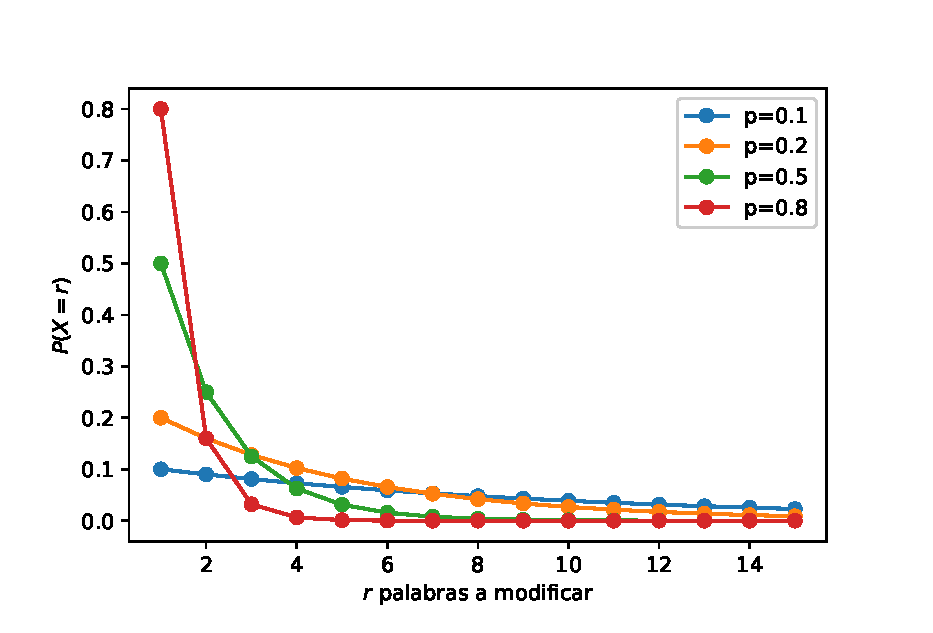
\includegraphics[width=\textwidth]{sections/figures/geometric_pmf.eps}
    \caption{Función de masa para la distribución geométrica con diferentes valores de probabilidad.}
    \label{fig:geom}
\end{figure}

\subsection{Etiquetado de partes de la oración}
El proceso de selección debe cuidar la modificación de ciertas partes de la oración, por un lado, evitar perder la interpretación original y por otro intentar conservar el estilo de la frase original. Por tal motivo, cada frase es etiquetada asignando a cada palabra su etiqueta POS (\textit{part of speech}) correspondiente. La tabla \ref{table:pos} muestra un ejemplo del etiquetado aplicado. Gracias al etiquetado, las palabras a reemplazar solo son aquellas que están más fuertemente asociadas al contenido de la frase, es decir, solo se seleccionan aquellas palabras con funciones gramaticales de: sustantivo, adjetivo, verbo y/o adverbio.


\begin{table}[h]
\caption{Ejemplo de etiquetado de partes de la oración.} \label{table:pos}
\begin{center}
\begin{tabular}{lllllll}
\hline
\textbf{Secuencia} & \textit{I} & \textit{am} & \textit{running} & \textit{out} & \textit{of} & \textit{ideas} \\ \hline
Etiqueta           & PRP        & VBP         & VBG              & IN           & IN          & NNS            \\ \hline
Equivalencia       & Pronombre  & Verbo       & Verbo            & Preposición  & Preposición & Sustantivo     \\ \hline
\end{tabular}
\end{center}
\end{table}

\subsection{Exclusión de palabras importantes}

Además de las palabras funcionales, también es deseable mantener palabras que aportan información para la tarea de clasificación que se desea realizar, por lo tanto, la primera propuesta consiste en evitar seleccionar, entre las palabras a reemplazar, aquellas palabras dependientes a la clase del documento. 

Para este proceso, recurrimos a la técnica de selección de características conocida como prueba de independencia $\chi^2$ (chi cuadrada). En estadística, la prueba $\chi^2$ es aplicada para comprobar la independencia de dos eventos, donde los eventos $A$ y $B$ son definidos a ser independientes si $P(AB)= P(A)P(B)$ o, equivalente, $P(A|B)=P(A)$ y $P(B|A)=P(B)$. En la selección de características para la clasificación de textos, los dos eventos son: \textit{ocurrencia del término} y \textit{ocurrencia de la clase}. Posteriormente se ordenan los términos de mayor a menor respecto a la ecuación \ref{eq:chi2}.

\begin{equation}
    \label{eq:chi2}
    \chi^2(D, t, c)= \sum_{e_t \in {0,1} }^{} \sum_{e_c \in {0,1} }^{} \frac{(N_{e_t e_c} - E _{e_t e_c})^2}{E_{e_t e_c}}
\end{equation}

El término $e_t$ indica la ausencia o presencia del término $t$ en el documento, similarmente el término $e_c$ indica si el documento se encuentra en la clase $c$. $N$ es la frecuencia observada en $D$ y $E$ es la frecuencia esperada. $\chi^2$ mide por cuanto los conteos esperados $E$ y los conteos observados $N$ se desvían de cada uno. Un valor alto de $\chi^2$ indica que la hipótesis de independencia, la cual implica que los conteos esperados y observados son similares, es incorrecta. Si los dos eventos son dependientes, entonces la ocurrencia del término hace la ocurrencia de la clase más probable (o menos probable), entonces el término debería ser seleccionado como relevante.

A través de este método se identifican todas aquellas palabras dependientes de la clase y, por ende, de relevancia para la tarea de clasificación. Dada la importancia de estas palabras se evitará reemplazarlas, excluyéndolas del proceso de selección de palabras a reemplazar.

\section{Reemplazo de palabras seleccionadas}

Una vez identificadas las palabras a reemplazar, el siguiente paso es, mediante la consulta de alguna fuente de conocimientos externa, buscar palabras candidatas similares a la palabra que se desea reemplazar. En \citep{zhang2015character} proponen consultar un tesauro con el objetivo de obtener los sinónimos de una palabra, sin embargo, el vocabulario contenido en el tesauro puede ser muy limitado o demasiado formal para el contexto del texto a aumentar. 

Una alternativa es buscar palabras similares a través de representaciones distribucionales de las palabras. La idea general de las representaciones distribucionales es codificar los \textit{tokens} de un vocabulario de tamaño finito $|V|$, en un vector que lo represente en espacio de palabras. La principal intuición de este enfoque es que deberá existir algún espacio $n$-dimensional, tal que $n<|V|$, donde codificar toda la semántica de un idioma. Cada dimensión codificará algún tipo de información, por ejemplo: las dimensiones semánticas podrían indicar el tiempo de conjugación (pasado, presente o futuro), de conteo (singular o plural) y género (masculino o femenino). En la subsección 2.2.4 se describen los modelos del estado del arte que siguen esta metodología.

El presente trabajo explora dos enfoques utilizando este recurso, la siguiente sección explica ambos enfoques.

\subsection{Similitud relacional}

Las representaciones distribucionales calculadas utilizando redes neuronales son muy interesantes debido a que los vectores aprendidos codifican muchas regularidades lingüísticas y patrones \citep{mikolov2013distributed}. Una de estas regularidades es la sinonimia y puede ser recuperada mediante alguna medida de distancia entre una palabra objetivo $w$ y el resto del vocabulario $V$. Esto se puede observar en la figura \ref{fig:word_plot}, en la cual se proyectan los vectores correspondientes a las palabras en un plano de dos dimensiones. En la figura, se observan las distancias entre palabras relacionadas con la palabra \textit{depresión} las cuales aparecen cercanas a una palabra, cuyo significado es más contrastante como la palabra \textit{feliz}. 

\begin{figure}[!hbt]
    \centering
  \includegraphics[scale=0.7]{sections/figures/word_plot.eps}
    \caption{Ejemplo comparando las distancias entre las proyecciones de los vectores de  palabras relacionadas a la palabra \textit{depresión} en contraste a la palabra \textit{feliz}.}
    \label{fig:word_plot}
\end{figure}

\subsubsection{Reemplazo por similitud relacional coseno}

La primera propuesta de reemplazo utiliza las representaciones distribucionales para reemplazar una palabra en una secuencia, por una palabra similar o altamente relacionada (i.e., aparecen en contextos similares). Para realizar esto se recupera el vector de la palabra a reemplazar de un modelo preentrenado de vectores de palabras y se calcula la distancia respecto a cada vector (representación de una palabra) en el modelo preentrenado. En este caso, hemos usado la medida de similitud coseno, véase la ecuación \ref{eq:coseno}. Esta ecuación indica que para obtener la distancia coseno de dos vectores de palabras se debe hacer un producto punto entre los vectores ($\vec{w}$, $\vec{v}$) y dividir el resultado por la multiplicación de la magnitud de los mismos.

\begin{equation}
\label{eq:coseno}
    cos(\vec{w},\vec{v})=\frac{\vec{w} . \vec{v}}{||\vec{w}||||\vec{v}||} = \frac{\sum_{i=1}^{n}w_i v_i}{\sqrt{\sum_{i=1}^{n}(w_i)^2} \sqrt{\sum_{i=1}^{n}(v_i)^2} }
\end{equation}

Específicamente para encontrar el conjunto de palabras candidatas $W$, dada una palabra $w$ se buscan las $k$ palabras más similares a $w$ de acuerdo con la ecuación \ref{eq:cosmax}.

\begin{equation}
    \label{eq:cosmax}
    argmax_{v \in V} (cos(\vec{w}, \vec{v}))
\end{equation}

Donde $\vec{v}$ es la representación vectorial de cada palabra en el vocabulario $V$ de vectores preentrenados y $\vec{w}$ es la representación vectorial de la palabra a sustituir. Una alta similitud coseno (cercana a 1) significa que los vectores comparten una dirección muy similar y por lo tanto hay una mayor probabilidad que las palabras sean utilizadas en los mismos contextos. En la tabla \ref{table:ejemplos_xi} se muestra el ejemplo de una secuencia, aumentada mediante este método, las palabras en negritas no se modifican debido a que son palabras con alta puntuación $\chi^2$ y en cursiva son resaltadas las palabras que se reemplazaron de la secuencia original. En el ejemplo la palabra \textit{morning} tiene como palabras candidatas las palabras:\textit{ sunday, afternoon y evening}. Aunque estas palabras no representan sinónimos de \textit{morning}, si conservan la misma etiqueta POS manteniendo el estilo de la secuencia original. 

\begin{table}[hbt!]
\caption{Ejemplos del aumento de datos, para el método con restricción $\chi^2$ y sustitución por similitud relacional.} 
\label{table:ejemplos_xi}
\centering
\begin{tabular}{ll}
\hline
                  & \textbf{Secuencia}                                                        \\ \hline
\textbf{Original} & \textbf{just} waking up every morning and \textbf{talking} to \textbf{my} gf \\ \hline
Aumentada         & just waking up every \textit{sunday} and talking to my gf \\ \hline
Aumentada         & just waking up every \textit{afternoon} and talking to my gf \\ \hline
Aumentada         & just \textit{woke} up every \textit{evening} and talking to my gf  \\ \hline
\end{tabular}

\end{table}


\subsubsection{Reemplazo por relaciones equivalentes}
Una de las características deseables en el aumento de datos es agregar un grado de diversidad o variabilidad en nuestros datos, sin embargo, al utilizar las representaciones distribucionales encontramos que las palabras con alta similitud coseno a una palabra, son por lo general variaciones pequeñas de esta misma palabra, por ejemplo, en la figura \ref{fig:analogia} lo más cercano a \textit{llorar} es \textit{llorando}. En este caso notamos que la diversidad deseada no se logra. 
Otro problema encontrado al calcular la similitud coseno entre dos palabras, dados sus vectores, es encontrar que palabras como \textit{llorar} y \textit{reir} suelen ser similares. Esto sucede porque ambas palabras ocurren en contextos de uso similares. Sin embargo, no deseamos hacer este tipo de sustituciones ya que sustituir una palabra por su antónimo (en lugar de un sinónimo) podría causar que la etiqueta original del documento se pierda.
\begin{figure}[!hbt]
\centering
\includegraphics[width=0.7 \textwidth]{sections/figures/analogia.png}
\caption{Palabras que ocurren en contextos de uso similares tienen una similitud relacional alta, incluyendo el caso de antónimos, por ejemplo \textit{llorar} vs \textit{reír} }
\label{fig:analogia}
\end{figure}

Para resolver este problema, explotamos la similitud relacional entre pares de palabras. Por ejemplo, al recuperar las palabras más similares a la palabra \textit{llorar}, encontramos: reír y llorando. Si sumamos el vector de la palabra \textit{llorar} con el vector de la palabra \textit{frustrado} podemos encontrar entre las palabras más cercanas: \textit{chillido} y \textit{enojo}, tal como se muestra en la figura \ref{fig:analogia}. De esta forma, mediante la aritmética de vectores podemos descubrir relaciones no tan obvias, y con ello crear una mayor diversidad en el vocabulario. Estas relaciones han sido previamente demostradas en \citep{mikolov2013linguistic}, junto con relaciones como singular - plural, adjetivos posesivo - no posesivo, base - comparativo, base - superlativo. Por  supuesto, se trata de una aproximación con la cual se ha alcanzado exactitudes de hasta un 41\%. 

En un contexto de aumento de datos asumimos que existe una relación entre la etiqueta de la clase y las palabras de una secuencia en un documento de esa clase. Para observar esta relación empleamos pares de palabras, intentando identificar analogías. Por ejemplo, se busca encontrar un segundo par de palabras que presente una relación análoga entre las palabras \textit{deprimido} (etiqueta de la clase) y \textit{llorar} (palabra de una secuencia perteneciente a la clase). En este caso suponemos que existe una relación entre \textit{deprimido} y \textit{llorar}; el siguiente paso es buscar una relación similar entre un sinónimo de \textit{deprimido}, puede ser \textit{frustrado}, y una palabra $v$ que desconocemos. Estas relaciones se muestran en la figura \ref{fig:analogia} mediante una línea punteada. 

 \begin{equation}
    \label{eq:grl_ejemplo}
     v \approx  llorar-deprimido+frustrado
 \end{equation}


De manera general para el aumento de datos proponemos expresar una analogía de la forma `` $w_{label}$ es a $w$ como $w_{syn}$ es a $v$", resolviendo la ecuación \ref{eq:grl_analogia} mediante aritmética de vectores.

 \begin{equation}
    \label{eq:grl_analogia}
    \vec{v} \approx \vec{w}-\vec{w_{label}}+\vec{w_{syn}}
\end{equation}
 
La ecuación \ref{eq:grl_ejemplo} resulta de sustituir en la ecuación \ref{eq:grl_analogia} las palabras involucradas para el aumento de datos. 
Siendo $\vec{w}$, $\vec{w_{label}}$  y $\vec{w_{syn}}$ las representaciones vectoriales de la palabra $w$ a reemplazar, la etiqueta de la clase a aumentar $w_{label}$ y un sinónimo de la etiqueta de la clase a aumentar $w_{syn}$. El vector $\vec{v}$ es la representación vectorial de la palabra a encontrar. Se busca que la palabra $v$ sea muy similar a $w$ pero orientada en el contexto del sinónimo $w_{syn}$. Es decir, el objetivo principal es encontrar palabras candidatas $v$ que comparten la misma relación reflejada entre \textit{llorar - deprimido} pero no necesariamente similar a \textit{llorar}.

 La ecuación \ref{eq:grl_analogia} es una forma directa para resolver preguntas de analogía. En \citep{mikolov2013linguistic}, propusieron este método nombrándolo método de compensación de vectores, en este método se asume que las relaciones semánticas entre palabras están presentes como una compensación de vectores, así que, en el espacio de características, todos los pares de palabras compartiendo una relación en particular están relacionadas por la misma constante de compensación. La variable $\vec{v}$ es la representación del espacio continuo de la palabra que esperamos sea la mejor respuesta. Claramente no existe ninguna palabra en la posición exacta, así que se busca la palabra cuyo vector tenga la mayor similitud coseno a $\vec{v}$. Resultando en:

\begin{equation}
\label{eq:3cosadd}
    arg max_{\vec{v}\in V}( cos (\vec{v}, \vec{w}-\vec{w_{label}}+\vec{w_{syn}}))
\end{equation}

Antes de aplicar la operación en \ref{eq:3cosadd}, todos los vectores son normalizados al vector unitario. Bajo esta normalización, dicha ecuación se puede expandir como en \ref{eq:3cosadd2}

\begin{equation}
\label{eq:3cosadd2}
    arg max_{\vec{v}\in V}( cos(\vec{v}, \vec{w}) - cos(\vec{v}, \vec{w_{label}}) + cos(\vec{v}, \vec{w_{syn}}) )
    \end{equation}

El objetivo anterior busca encontrar una palabra similar a $w$ (la palabra que deseamos reemplazar), diferente de $w_{label}$ (la etiqueta de la clase a aumentar) y similar a $w_{syn}$ (un sinónimo de la etiqueta a aumentar). Al maximizar este objetivo \citep{mikolov2013distributed} comprobó que se puede recuperar hasta un 53\% de las analogías en el conjunto de datos MSR\footnote{research.microsoft.com/en-us/projects/rnn/}. Aun así, \citep{levy2014linguistic} encontró que la formulación en \ref{eq:3cosadd2} permite que un término suficientemente grande domine la expresión y como consecuencia obtener resultados incorrectos, para alcanzar un mejor balance entre los diferentes aspectos de similitud, propusieron la ecuación 3COSMUL ( \ref{eq:3cosmul}). Esta fórmula amplifica las diferencias entre pequeñas cantidades y las reduce entre las grandes. Mediante esta fórmula se logro recuperar el 59\% de las analogías en el conjunto MSR.

\begin{equation}
    \label{eq:3cosmul}
    arg max_{\vec{v}\in V} \frac{ cos(\vec{v}, \vec{w}) cos(\vec{v}, \vec{w_{sym}})}
    { cos(\vec{v}, \vec{w_{label}})+ \epsilon}
\end{equation}

Bajo este nuevo escenario, primero se obtiene la similitud de la palabra $w$ a ser reemplazada y una palabra $v$ en el vocabulario, el resultado es multiplicado por la similitud de la palabra $v$ y un sinónimo de la etiqueta de la clase a aumentar $w_{syn}$. Con esto se espera amplificar la similitud entre $v$ y la palabra a reemplazar $w$ por la magnitud de la similitud entre $v$ y $w_{syn}$. El denominador busca incrementar el resultado anterior si existe disimilitud entre $v$ y la etiqueta $w_{label}$ de la palabra a aumentar. 
Finalmente, sustituyendo las representaciones vectoriales de $v$ para cada palabra en el vocabulario $V$, $w$, $w_{label}$ y $w_{syn}$ en la formula \ref{eq:3cosmul} obtenemos las palabras candidatas $W$ con mayor puntuación. Antes de obtener el resultado de \ref{eq:3cosmul}, las similitudes coseno son transformadas en el rango [0,1] utilizando $\frac{x+1}{2}$ y $\epsilon$ es un número muy pequeño usado para evitar la división por cero.

En la tabla \ref{table:ejemplos_equiv}, se presenta un ejemplo de este método de aumento, el cual hemos nombrado de \textbf{reemplazo por relaciones equivalentes}.
En la primera columna se indica la etiqueta de la clase a aumentar \textit{depressed} y sus sinónimos: \textit{anxious, frustrated, unhappy, despondent y discouraged}; por cada sinónimo se obtiene una secuencia aumentada.

\begin{table}[hbt!]
\caption{Ejemplos del aumento de datos para el método basado en reemplazo por relaciones equivalentes.} 
\label{table:ejemplos_equiv}
\begin{center}
\resizebox{\columnwidth}{!}{%

\begin{tabular}{ll}
\hline
 & \textbf{Secuencia}                                        \\ \hline
\textbf{Original}                                                & oh man this sucks it maybe looks funny from outside but it just looks like hell from here              \\ \hline
\begin{tabular}[c]{@{}l@{}}depressed-\\ anxious\end{tabular}     & oh man this sucks it maybe look funny from outside but it just \textit{looked} like \textit{wait} from here              \\ \hline
\begin{tabular}[c]{@{}l@{}}depressed-\\ frustrated\end{tabular}  & oh man this suck it \textit{perhaps} looks \textit{stupid} from outside but it just looks like hell from here            \\ \hline
\begin{tabular}[c]{@{}l@{}}depressed-\\ unhappy\end{tabular}     & oh \textit{woman }this sucks it maybe \textit{looking} funny from outside but it just looks like hell from here          \\ \hline
\begin{tabular}[c]{@{}l@{}}depressed-\\ despondent\end{tabular}  & oh man this \textit{pisses} it though looks \textit{humourous }from outside but it just \textit{dashing} like \textit{purgatory }from here \\ \hline
\begin{tabular}[c]{@{}l@{}}depressed-\\ discouraged\end{tabular} & oh \textit{god} this \textit{sucked} it \textit{anyway} \textit{seems humorous} from outside but it just think \textit{like bother} from here       \\ \hline
\end{tabular}


}

\end{center}
\end{table}


\subsubsection{Reemplazo por relaciones contrarias}

En escenarios desbalanceados el aumento de datos puede llevarnos a un sobremuestreo de la clase minoritaria, generalmente la clase de interés. Los métodos presentados anteriormente fueron diseñados para aumentar esta clase minoritaria (a la cual también nos referimos como clase positiva). Sin embargo, una desventaja de hacer esto es que el modelo de aprendizaje se restringe al vocabulario de la clase positiva lo que provoca un sobreajuste. En un intento de contrarrestar esta situación, se propone un método que incorpora documentos seleccionados de la clase negativa a la clase positiva. Por supuesto, para ello es necesario realizar una transformación de las instancias negativas.

Para llevar a cabo esta transformación adaptamos el método propuesto por \citep{zhang2019integrating}. En dicho método se aborda el problema de  \textit{zero-shot text classification}, en esa situación se toma un documento de una clase etiquetada y lo \textit{traduce} para considerarlo como instancia de una clase totalmente nueva. Este método no tiene ninguna restricción respecto sobre las palabras a reemplazar, en nuestro caso hemos incluido un criterio de selección para guiar la generación de los nuevos documentos los cuales servirán para aumentar el conjunto de la clase de interés.   

La idea básica de la transformación recae en el mismo método visto en la sección anterior. Sin embargo, los pares de palabras usadas para representar la analogía son escogidas para identificar palabras con una relación opuesta o \textit{contraria}. Por ejemplo, en el caso de la tarea de detección de depresión, asociaremos la palabra \textit{``feliz"} como representativa de la clase \textit{no deprimidos}  y la palabra \textit{``deprimido"} para la clase \textit{deprimidos}. Ahora bien, reemplazaremos palabras de documentos de la clase \textit{no deprimidos} por palabras que presentan la relación opuesta deseada, la cual es guiada por el par de palabras \textit{feliz} vs \textit{deprimido}. 

En la ecuación \ref{eq:contraria} se asume que existe una relación entre la palabra a reemplazar (novia) y la etiqueta de la clase no depresiva (feliz), buscamos una palabra $v$ que comparte una relación similar entre (novia) y la etiqueta que deseamos aumentar (feliz).

\begin{equation}
    \label{eq:contraria}
    v \approx novia - feliz + deprimido.
\end{equation}
Sustituyendo las palabras de \ref{eq:contraria}: novia, feliz y deprimido por su representación vectorial en \ref{eq:3cosmul} como $\vec{w}$, $\vec{w_{label}}$ y $\vec{w_{syn}}$ respectivamente.
 

La tabla \ref{table:ejemplos_contraria} presenta ejemplos del aumento basado en relaciones contrarias, las palabras relacionadas con un contexto feliz, son llevadas a un contexto contrario. Por ejemplo, el verbo \textit{``talked"} es reemplazado por \textit{``complained"} y \textit{``bothered"}. Similar al método anterior se utilizan los sinónimos de la palabra \textit{depressed} para el aumento.

\begin{table}[hbt!]
\caption{Ejemplos del aumento de datos para el método basado en relaciones opuestas.} 
\label{table:ejemplos_contraria}
\begin{center}

\begin{tabular}{ll}
\hline
\rowcolor[HTML]{EFEFEF} 
\textbf{Método} & \textbf{Secuencia}                                           \\ \hline
\rowcolor[HTML]{FFFFFF} 
Sin Aumento     & i connected with a girl we sat up and talked all night       \\ \hline
\rowcolor[HTML]{FFFFFF} 
Opuesta       & i disconnected with a girl we sat up and talked all night    \\ \hline
\rowcolor[HTML]{FFFFFF} 
Opuesta       & i connected with a girl we sat up and complained all night   \\ \hline
\rowcolor[HTML]{FFFFFF} 
Opuesta       & i connected with a boy we complained up and talked all night \\ \hline
\rowcolor[HTML]{FFFFFF} 
Opuesta       & i dispirited with a girl we sat up and talked all night      \\ \hline
\rowcolor[HTML]{FFFFFF} 
Opuesta       & i connected with a shy we dismayed up and bothered all night \\ \hline
\end{tabular}

\end{center}
\end{table}
\chapter{Configuración experimental y resultados}
En este capítulo se presenta la configuración experimental y el detalle de los conjuntos de datos empleados, además de los parámetros elegidos para la construcción de los diferentes clasificadores para la evaluación del método propuesto, al final se presenta un análisis de los resultados y se comparan las diferentes estrategias de aumento de datos. Adicionalmente, para poder reproducir los resultados, este proyecto está públicamente disponible en github\footnote{github.com/v1ktop/data\_augmentation\_for\_author\_profiling}.



\section{Configuración experimental}


La configuración experimental sigue  un enfoque supervisado. En la cual se cuenta con un conjunto de historiales de usuario, los cuales pueden verse como un sólo documento, a este documento $X$ le corresponde su etiqueta correspondiente $y \in Y$  en una relación uno a uno. En todos los conjuntos de datos usados se trata únicamente de dos clases, es decir, se trata de una clasificación binaria ($|Y| = 2$). 

La metodología empleada está compuesta de 4 fases:  preprocesamiento, aumento de datos, entrenamiento y evaluación. En el preprocesamiento se realizan las modificaciones necesarias para normalizar los documentos, además de segmentarlos y filtrarlos (tal como se explica en párrafos posteriores); posteriormente se pasa a la etapa de aumento de datos. Una vez con que se han aumentado los datos de entrenamiento se construye un modelo de clasificación, a través de un algoritmo de aprendizaje máquina (en específico es de nuestro interés los métodos de redes profundas). Finalmente, se evalúa el modelo de clasificación sobre un conjunto de datos que no ha sido aumentado ni utilizado en la búsqueda de parámetros durante el entrenamiento, únicamente es preprocesado de la misma forma que los datos de entrenamiento. La figura \ref{fig:metodologia} muestra las diferentes fases descritas.

\begin{figure}[h]
    \includegraphics[width=\textwidth]{sections/figures/diagrama_general.png}
    \caption{Diagrama general de la configuración experimental}
    \label{fig:metodologia}
\end{figure}

\subsection{Conjunto de datos}

\textbf{Depresión 2018 y Anorexia}: Con el propósito de estudiar la detección temprana de depresión y anorexia, los autores \citep{Losada2018} recopilaron publicaciones de diversos usuarios de la red social Reddit. Para cada usuario la colección contiene una secuencia de publicaciones en orden cronológico. Este conjunto de datos se caracteriza por tener una gran cantidad de texto pero con muy pocos usuarios, como se puede observar en la figura \ref{fig:erisk_freq}. Hay dos categorías para cada usuario en cada tarea. El número de usuarios total en cada conjunto se presenta en la tabla \ref{table:original_users}. Dado que se trabaja con conjuntos de datos muy desbalanceados el aumento de datos solo se aplica sobre la clase de interés o clase positiva.

\textbf{Depresión 2019}: Presentado en la tareas eRisk 2019 \cite{Losada2019}, a diferencia de la edición 2018 en esta ocasión el objetivo es predecir los niveles de depresión de un usuario (mínima, media, moderada, severa). Con el objetivo de que los resultados sean comparables en este trabajo se redujo el problema a una clasificación binaria como se trato con el conjunto del 2018; para esto los usuarios con depresión media a severa se tomaron como ejemplos de la clase positiva.

Para el entrenamiento solo se consideraron 16 usuarios para la clase positiva como se muestra en la tabla \ref{table:original_users}, para obtener usuarios de la clase negativa se tomaron los etiquetados como negativos en el conjunto de entrenamiento del eRisk 2018. Finalmente el conjunto de test, solo se dividió en dos clases quedando 60 positivos y 10 negativos (deprimidos y no deprimidos respectivamente).
\begin{table}[!hbt]
\caption{Número de usuarios en los conjuntos de datos y número de secuencias con 64 palabras. Los números resaltados en negritas representan el número de historiales.} \label{table:original_users}

\begin{center}

\begin{tabular}{llll}
\hline
\rowcolor[HTML]{FFFFFF} 
\textbf{Usuarios}                                           & \textbf{Entrenamiento}                       & \textbf{Evaluación}                          & \textbf{Vocabulario}                                         \\ \hline
\rowcolor[HTML]{EFEFEF} 
\textit{Conjunto 1: Depresión 2018}                         & \multicolumn{1}{c}{\cellcolor[HTML]{EFEFEF}} & \multicolumn{1}{c}{\cellcolor[HTML]{EFEFEF}} &                                                              \\ \hline
\rowcolor[HTML]{FFFFFF} 
deprimido                                                   & \textbf{135} - 31,396                                 & \textbf{79} - 25,967                                  &                                                              \\ \hline
\rowcolor[HTML]{FFFFFF} 
no-deprimido                                                & \textbf{752} - 227,189                                & \textbf{741} - 272,703                                &                                                              \\ \hline
\rowcolor[HTML]{FFFFFF} 
\textbf{Total}                                              & \textit{\textbf{887} - 258,585}                       & \textit{\textbf{820} - 298,670}                       & \multicolumn{1}{c}{\cellcolor[HTML]{FFFFFF}\textit{202,151}} \\ \hline
\rowcolor[HTML]{EFEFEF} 
\cellcolor[HTML]{EFEFEF}\textit{Conjunto 2: Depresión 2019} &                                              &                                              &                                                              \\ \hline
\rowcolor[HTML]{FFFFFF} 
deprimido                                                   & \textbf{16} - 5,731                                   & \textbf{60} - 18,534                                  &                                                              \\ \hline
\rowcolor[HTML]{FFFFFF} 
no-deprimido                                                & \textbf{752} - 227,189                                & \textbf{10} - 5,011                                   &                                                              \\ \hline
\rowcolor[HTML]{FFFFFF} 
\textbf{Total}                                              & \textit{\textbf{768} - 232,920}                       & \textit{\textbf{70} - 23,545}                         & \multicolumn{1}{c}{\cellcolor[HTML]{FFFFFF}\textit{195,047}}    \\ \hline
\rowcolor[HTML]{EFEFEF} 
\textit{Conjunto 3: Anorexia}                               & \multicolumn{1}{c}{\cellcolor[HTML]{EFEFEF}} & \multicolumn{1}{c}{\cellcolor[HTML]{EFEFEF}} &                                                              \\ \hline
\rowcolor[HTML]{FFFFFF} 
con anorexia                                                & \textbf{61} - 23,335                                  & \textbf{73} - 16,751                                  &                                                              \\ \hline
\rowcolor[HTML]{FFFFFF} 
sin-anorexia                                                & \textbf{411} - 107,239                                 & \textbf{742} - 254,640                                &                                                              \\ \hline
\rowcolor[HTML]{FFFFFF} 
\textbf{Total}                                              & \textit{\textbf{472} - 130,574}                       & \textit{\textbf{815} - 271,391}                       & \multicolumn{1}{c}{\cellcolor[HTML]{FFFFFF}\textit{131,264}}  \\ \hline
\end{tabular}

\end{center}

\end{table}


\begin{table}[!hbt]
\caption{Número de usuarios en los conjuntos de datos y número de secuencias con 64 palabras después del pre-procesamiento, realizando el filtro. Los números resaltados en negritas representan el número de historiales comparado con el número de secuencias} \label{table:filter_users}

\resizebox{\textwidth}{!}{%

\begin{tabular}{llll}
\hline
\rowcolor[HTML]{FFFFFF} 
\textbf{Usuarios}                   & \textbf{Entrenamiento}                       & \textbf{Evaluación}                          & \textbf{Vocabulario}                                         \\ \hline
\rowcolor[HTML]{EFEFEF} 
\textit{Conjunto 1: Depresión 2018} & \multicolumn{1}{c}{\cellcolor[HTML]{EFEFEF}} & \multicolumn{1}{c}{\cellcolor[HTML]{EFEFEF}} &                                                              \\ \hline
\rowcolor[HTML]{FFFFFF} 
deprimido                           & \textbf{135} - 24,483                                 & \textbf{79} - 25,967                                  &                                                              \\ \hline
\rowcolor[HTML]{FFFFFF} 
no-deprimido                        & \textbf{744} - 98,783                                 & \textbf{741} - 272,703                                &                                                              \\ \hline
\rowcolor[HTML]{FFFFFF} 
\textbf{Total}                      & \textit{\textbf{879} - 123,266}                       & \textit{\textbf{820} - 298,670}                       & \multicolumn{1}{c}{\cellcolor[HTML]{FFFFFF}\textit{104,800}} \\ \hline
\rowcolor[HTML]{EFEFEF} 
\textit{Conjunto 2: Depresión 2019} & \multicolumn{1}{c}{\cellcolor[HTML]{EFEFEF}} & \multicolumn{1}{c}{\cellcolor[HTML]{EFEFEF}} &                                                              \\ \hline
\rowcolor[HTML]{FFFFFF} 
deprimido                           & \textbf{16} - 5,731                                   & \textbf{60} - 18,534                                  &                                                              \\ \hline
\rowcolor[HTML]{FFFFFF} 
no-deprimido                        & \textbf{746} - 125,823                                & \textbf{10} - 5,011                                   &                                                              \\ \hline
\rowcolor[HTML]{FFFFFF} 
\textbf{Total}                      & \textit{\textbf{762} - 131,554}                       & \textit{\textbf{70} - 23,545}                         & \multicolumn{1}{c}{\cellcolor[HTML]{FFFFFF}\textit{118,668}}    \\ \hline
\rowcolor[HTML]{EFEFEF} 
\textit{Conjunto 2: Anorexia}       & \multicolumn{1}{c}{\cellcolor[HTML]{EFEFEF}} & \multicolumn{1}{c}{\cellcolor[HTML]{EFEFEF}} &                                                              \\ \hline
\rowcolor[HTML]{FFFFFF} 
con anorexia                        & \textbf{61}-15,657                                    & \textbf{73}-16,751                                    &                                                              \\ \hline
\rowcolor[HTML]{FFFFFF} 
sin-anorexia                        & \textbf{405}-58,837                                  & \textbf{742}-254,640                                  &                                                              \\ \hline
\rowcolor[HTML]{FFFFFF} 
\textbf{Total}                      & \textit{\textbf{466}-{74,494}}                         & \textit{\textbf{815}-271,391}                         & \multicolumn{1}{c}{\cellcolor[HTML]{FFFFFF}\textit{80,964
}} \\ \hline
\end{tabular}

}

\end{table}



%[!htbp]
\begin{figure}[!ht]
    
    \begin{subfigure}[b]{0.5\textwidth}
        \includegraphics[width=\textwidth]{sections/figures/length_dist.eps}
        \caption{Depresión}
    \end{subfigure}
    \hfill
    \begin{subfigure}[b]{0.5\textwidth}
        \includegraphics[width=\textwidth]{sections/figures/length_dist_anorexia.eps}
        \caption{Anorexia}
    \end{subfigure}
    \caption{Distribución del numero de palabras en los conjuntos de datos estudiados}
    \label{fig:erisk_freq}
\end{figure}

%% Agregar las distribución del conjunto anorexia


\subsection{Pre-procesamiento}

Dado que los documentos extraídos de redes sociales no siguen un lenguaje formal y además de texto existen direcciones de páginas web que los usuarios comparten, emoticonos y cáracteres especiales, entre otros; es necesario que antes del aumento de datos exista un preprocesamiento de los textos como una forma de reducir el ruido de los documentos originales.

Los pasos del procesamiento seguido son los siguientes:

 \begin{enumerate}
     \item Normalización: Se identifican las páginas web en el texto y se reemplazan mediante la etiqueta http\_
     \item Tokenización: Utilizando la herramienta NLTK se remueve de cada texto signos de puntuación y cáracteres especiales.
     \item Segmentación: Los documentos originales son segmentados en pequeños fragmentos. Es decir, cada historial de usuario se fragmenta en secuencias de 64 palabras  (véase la siguiente sección). 
     %\item Filtro: En la clasificación de documentos no todo el contenido del texto esencial para determinar la categoría a la cual pertenece, es decir existe cierta combinación de palabras que sirven para discriminar la clase. Para determinar estas palabras se emplea el método de selección de características denominado Chi-cuadrada.
     \item Filtrado: Solo se conservan segmentos identificados como importantes para la clasificación (véase la siguiente sección).
 \end{enumerate}



\subsubsection{Segmentación y filtrado}
Con el proposito de que el aumento de datos pueda ser proporcional independientemente de la longitud del documento original. Cada documento se dividió en segmentos de 64 palabras\footnote{Este parámetro se determinó de manera empírica.}. Posteriormente se filtró el conjunto de entrenamiento para conservar solo los segmentos importantes para realizar la clasificación. Es decir, se identificaron aquellos fragmentos con la mayor cantidad de palabras discriminantes. Para ello se identificaron las  palabras más discriminantes dentro del vocabulario del conjunto de entrenamiento mediante la técnica de selección de características $\chi^2$. Posteriormente se conservaron aquellos fragmentos  que contengan un determinado número de palabras con alta puntuación $\chi^2$. 

Específicamente solo se seleccionaron términos estadísticamente significativos al nivel 0.001, equivalente a una puntuación $\chi^2 > $ 10.83 con un grado de libertad. En la tabla \ref{table:filter_users} se muestran los números de usuarios y secuencias obtenidas después de aplicar este filtro; para el conjunto de depresión el criterio de selección fue que la secuencia contuviera al menos 20 palabras de 1071 palabras con alta puntuación, y para el conjunto de anorexia 15 palabras de 1032. Como puede observarse en ambos casos se trata de umbrales altos. Esto se debe principalmente a que en las palabras con alta puntuación están presentes palabras vacías, palabras que tradicionalmente se eliminan para tareas de clasificación temática. No obstante, en nuestro caso,  se trata de una tarea donde el estilo es importante (p.e. uso de pronombres personales).



\subsection{Configuración de los métodos propuestos}

Para comprobar la efectividad del método propuesto se experimenta con  7 configuraciones diferentes: 2 líneas base, 2 métodos del estado del arte y 3 métodos propuestos. Además de esto se introduce un parámetro $n$ para observar el grado pertinente del aumento de datos, el cual indica el número de documentos nuevos aumentados, tomando valores enteros en el rango $[1,10]$.


\subsubsection{Sin aumento de datos}
Este método es la primera línea base y solo consideran los datos originales filtrados para el entrenamiento de los modelos (véase la tabla \ref{table:filter_users}).

\subsubsection{Sobre muestreo}
Esta línea base, consiste en incrementar el número de ejemplos de la clase minoritaria; este método no implica alguna pérdida de información ya que ningún elemento es modificado o descartado. Sin embargo la única desventaja es, que el modelo de aprendizaje generado tiende a sobre ajustarse, debido a que no agrega variabilidad en los datos.

\subsubsection{Tesauro}
Este método del estado del arte fue propuesto por \citep{zhang2015character} y demostró mejoras de un 1 a 2\% en exactitud para la clasificación de opiniones. También fue implementado por \citep{wei2019eda} con algunas modificaciones obteniendo una mejora entre un 1 y 2\% en comparación de no hacer aumento de datos, otros trabajos que utilizan este método como referencia y han encontrado evidencia de que agrega una ganancia en los resultados de clasificación son: \citep{jungiewicz2019towards}, \citep{kumar2019submodular}, \citep{park2019self}.

Para decidir cuantas palabras reemplazar dada una secuencia de palabras, se utiliza el parámetro $p=$ 0.5 para calcular el valor de $r$ palabras a reemplazar, la selección de dichas palabras es aleatoria, el recurso externo para encontrar sinónimos es un tesauro (en este caso Wordnet\footnote{www.wordnet.princeton.edu/}), y finalmente en la fase de reemplazo, de las palabras candidatas, se selecciona el índice dado un número aleatorio $s$ generado de una distribución geométrica con parámetro $q=$ 0.5.

El propósito de este método es ser muy conservativo en la modificación del texto original y el número $s$ controla la diversidad del vocabulario que por lo generaPara decidir que palabras reemplazarempleada).

\subsubsection{Sustitución sin restricción y reemplazo mediante similitud coseno}
Diversos estudios sugieren utilizar vectores de modelos pre-entrenados como Word2Vec, Glove, entre otros; la idea es recuperar palabras que se utilizan en contextos similares, en lugar de sinónimos. 

Para decidir que palabras reemplazar se omiten palabras de paro y aquellas que no sean etiquetadas como sustantivos, adjetivos, verbos y adverbios; con el propósito de agregar mas variabilidad en los ejemplos el número $r$ es calculado con el parámetro $p=$ 0.2. En la fase de reemplazo las palabras más similares se seleccionan mediante similitud coseno, utilizándolas de mayor a menor en una selección sin reemplazo.

El modelo de vectores pre-entrenados para representar las palabras de una secuencia fue Glove\footnote{https://nlp.stanford.edu/projects/glove/} con 300 dimensiones \citep{pennington2014glove}. Este modelo fue pre-entrenado con la base de datos Common Crawl, con 42 millones de  tokens y 1.9 millones de palabras. 

Con este método se espera obtener mayor diversidad en el vocabulario en comparación a utilizar un tesauro y obtener palabras muy similares que se emplean en el mismo contexto.

\subsubsection{Sustitución con restricción $\chi2$  y reemplazo mediante similitud relacional}
A diferencia del método anterior, una vez calculado el número $r$ de palabras a reemplazar, se omiten las palabras con mayor puntuación $\chi^2$ con un nivel de significación estadística de 0.001. Con este método se espera conservar una combinación de estilo y contenido además de agregar variabilidad en los datos. 

\subsubsection{Reemplazo mediante similitud relacional equivalente}
En la fase de selección se fija el valor del parámetro $p=$ 0.2 y en la fase de reemplazo se utiliza la similitud relacional positiva; esto es obtener un vocabulario muy similar a la etiqueta de la clase pero no el mismo. Las relaciones buscadas se enlistan en la tabla \ref{table:etiquetas} para cada tarea de clasificación. Por ejemplo, para buscar las palabras candidatas a la palabra ``boyfriend", se utiliza la relación \textit{``depressed"} es a \textit{``boyfriend"} como \textit{``anxious"} es a \textbf{?}. 

\subsubsection{Reemplazo mediante similitud relacional contraria}
Este último método es similar al método anterior, lo único que cambia es la clase objetivo, en este caso se toman los documentos de clase opuesta (la clase negativa). Por ejemplo para buscar las palabras candidatas a la palabra ``boyfriend", se utiliza la relación \textit{``happiness"} es a \textit{``boyfriend"} como \textit{``anxious"} es a \textbf{?}. La tabla \ref{table:etiquetas} resume las etiquetas empleadas para realizar el aumento.


\begin{table}[!hbt]
\caption{Etiquetas utilizadas en el proceso de aumento para los métodos de similitud relacional.} \label{table:etiquetas}
\begin{center}

\begin{tabular}{llll}
\hline
\rowcolor[HTML]{C0C0C0} 
Conjunto           & Clase & Etiqueta  & Palabra relacionada \\ \hline
\textbf{Depresión} & 1     & depressed & anxious           \\ \hline
                   & 0     & happiness & frustrated        \\ \hline
                   &       &           & unhappy           \\ \hline
                   &       &           & despondent        \\ \hline
                   &       &           & discouraged       \\ \hline
\textbf{Anorexia}  & 1     & anorexic  & bulimic           \\ \hline
                   & 0     & healthy   & underweight       \\ \hline
                   &       &           & obese             \\ \hline
                   &       &           & malnourished      \\ \hline
                   &       &           & unhealthy         \\ \hline
\end{tabular}

\end{center}
\end{table}


\subsubsection{Ejemplos del aumento de datos}
En la tabla \ref{table:ejemplos_pos} se presentan diversos ejemplos de aumento, el método basado en tesauro agrega un vocabulario mas formal, en comparación con los basados en similitudes relacionales. El método basado en restricción $\chi^2$ conserva palabras importantes como ``feel", mientras que los otros no toman en consideración esto. Por otra parte el método basado en relaciones equivalentes agrega la palabra \textit{``unfortunate"} como una palabra relacionada a la palabra \textit{``unhappy"}.

La tabla \ref{table:ejemplos_contraria} presenta ejemplos del aumento basado en relaciones contrarias, las palabras relacionadas a un contexto feliz, son llevadas a un contexto contrario. Por ejemplo el verbo \textit{``talked"} es reemplazado por \textit{``complained"} y \textit{``bothered"}.
\begin{table}[hbt!]
\caption{Ejemplos del aumento de datos, las palabras resaltadas en negritas son las que resultaron afectadas después de la transformación.} 
\label{table:ejemplos_pos}
\begin{center}

\resizebox{\columnwidth}{!}{%
\begin{tabular}{ll}
\hline
\rowcolor[HTML]{EFEFEF} 
\textbf{Método} & \textbf{Secuencia}                                                            \\ \hline
\rowcolor[HTML]{FFFFFF} 
Sin Aumento     & a lot of the time i have trouble communicating why i feel so unhappy          \\ \hline
\rowcolor[HTML]{FFFFFF} 
Thesauro        & a lot of the time i \textbf{hold} trouble communicating why i feel \textbf{thusly infelicitous} \\ \hline
\rowcolor[HTML]{FFFFFF} 
Sin Restricción & a \textbf{lots} of the time i have trouble communicating why i \textbf{feeling} so unhappy      \\ \hline
\rowcolor[HTML]{FFFFFF} 
Restricción $\chi^2$ & a lot of the time i have \textbf{difficulty} \textbf{informing} why i feel so unhappy           \\ \hline
\rowcolor[HTML]{FFFFFF} 
Equivalencia    & a \textbf{much} of the \textbf{place} i have \textbf{troubles informing} why i \textbf{feeling} so \textbf{unfortunate}    \\ \hline
\end{tabular}
}
\end{center}
\end{table}

\begin{table}[hbt!]
\caption{Ejemplos del aumento de datos para el método basado en relaciones opuestas.} 
\label{table:ejemplos_contraria}
\begin{center}

\begin{tabular}{ll}
\hline
\rowcolor[HTML]{EFEFEF} 
\textbf{Método} & \textbf{Secuencia}                                           \\ \hline
\rowcolor[HTML]{FFFFFF} 
Sin Aumento     & i connected with a girl we sat up and talked all night       \\ \hline
\rowcolor[HTML]{FFFFFF} 
Opuesta       & i disconnected with a girl we sat up and talked all night    \\ \hline
\rowcolor[HTML]{FFFFFF} 
Opuesta       & i connected with a girl we sat up and complained all night   \\ \hline
\rowcolor[HTML]{FFFFFF} 
Opuesta       & i connected with a boy we complained up and talked all night \\ \hline
\rowcolor[HTML]{FFFFFF} 
Opuesta       & i dispirited with a girl we sat up and talked all night      \\ \hline
\rowcolor[HTML]{FFFFFF} 
Opuesta       & i connected with a shy we dismayed up and bothered all night \\ \hline
\end{tabular}

\end{center}
\end{table}

 
\subsection{Configuración de los modelos de aprendizaje}

Para evaluar el efecto del aumento de datos se utilizaron dos arquitecturas de aprendizaje profundo. Ambas son arquitecturas con resultados relevantes en tareas de clasificación de textos: una red LSTM bidireccional y una red convolucional CNN. Cada arquitectura tiene diferencias, por ejemplo, al considerar el aspecto secuencial inherente de un texto, en el caso de la red recurrente; o cuando se consideran subsecuencias como elementos aislados en el caso de la red convolucional.

A pesar de que el enfoque principal de este trabajo está enfocado al efecto del aumento de datos en redes neuronales profundas, también se realizaron experimentos en modelos tradicionalmente usados en la clasificación de textos. El objetivo es tener valores de referencia respecto a los métodos propuestos. 

Como métodos de clasificación tradicional, se usaron las Máquinas de Soporte Vectorial, considerando el desbalanceo o no al modificar el parámetro de regularización $c$. Nos referiremos al modelo que no considera el desbalanceo como SVM y cuando se considera lo indicamos como SVM-C. 


\subsubsection{Modelos lineales}
 El primer modelo es construido mediante una Máquina de Soporte Vectorial (SVM) con kernel lineal, la entrada es el historial completo de un usuario representado como un vector de características mediante el pesado \textit{tf-idf} y normalizado mediante la norma $l2$, las palabras de paro se mantienen y se utiliza todo el vocabulario extraído como características. 
 
 El segundo algoritmo utilizado, SVM-C,  es basado en el primer modelo, con la diferencia de que en este caso se modifica el parámetro de regularización $C$ y automáticamente se ajustan los pesos inversamente proporcional a la frecuencia de las clases en los datos de entrada de acuerdo la ecuación \ref{eq:weights_balance}
 
 \begin{equation}
 \label{eq:weights_balance}
     C = N/2c_n
 \end{equation}
 
 En donde $N$ es el número total de ejemplos y $c_n$ el número de ejemplos en la clase $c$.  

\subsubsection{Modelos basados en redes neuronales}

Con el objetivo principal de establecer las bases sobre en que tipo de arquitecturas es más recomendable realizar aumento de datos. Se implementan dos arquitecturas diferentes: una red Bidireccional LSTM (Bi-LSTM) y una red convolucional (CNN); teniendo en común la capa de entrada y capa de salida.

La \textbf{capa de entrada} recibe una secuencia de 64 palabras, cada palabra es representada por un vector de 300 dimensiones obtenido del modelo pre-entrenado FastText\footnote{https://fasttext.cc/docs/en/crawl-vectors.html} , si alguna palabra no está en el vocabulario, su vector es obtenido de la representación de sus n-gramas de caracteres. En el entrenamiento esta capa es estática para reducir el número de parámetros entrenables.

La \textbf{capa de salida} es una neurona que recibe como entrada la última capa oculta del modelo, la representación aprendida de los parámetros internos. Mediante la función sigmoide, ecuación \ref{eq:sigmoide}, se calcula la probabilidad de que la secuencia de palabras pertenezca a la clase 0 o a la clase 1.

\begin{equation}
    \label{eq:sigmoide}
    sigmoid(x) = \frac{1}{1+ e^{-x}}
\end{equation}

Para inicializar los pesos de la capa final correctamente, el \textit{bias} (sesgo) inicial se deriva de la ecuación \ref{eq:bias}.  Con la inicialización correcta la función de perdida inicial se debe aproximar a $ln(2)=$ 0.69314. 

\begin{equation}
\label{eq:bias}
\begin{split}
    p_0= \frac{pos}{pos+neg}= \frac{1}{1+e^{-b_0}}\\
    b_0=-log_e(\frac{1}{p_0-1})\\
    b_0=log_e(pos/neg)
\end{split}
\end{equation}

Configurando el sesgo inicial correctamente ayuda a la convergencia del modelo desde la primer época.

Derivado de la arquitectura presentada en  \citep{adhikari2019rethinking}, en la figura  \ref{fig:lstm_model}, se presenta la arquitectura empleada para el modelo Bi-LSTM, la red bidireccional se compone de dos redes LSTM con 256 neuronas cada una, posteriormente se aplica una capa de \textit{Dropout} con una tasa de 0.2 , una capa totalmente conectada con 256 unidades, una capa de \textit{Dropout} con una tasa de 0.2 y en la última capa una sola neurona activada mediante la función sigmoide \ref{eq:sigmoide}. Los nodos intermedios de las capas ocultas se activan con la función de activación Relu \ref{eq:RELU}. 
\begin{figure}[!hb]
    \centering
  \includegraphics[scale=0.25]{sections/figures/lstm_model.png}
    \caption{Arquitectura del modelo Bi-LSTM}
    \label{fig:lstm_model}
\end{figure}

%%Cambiar diagrama por uno mas censillo y mas abstracto

En la figura \ref{fig:cnn_model}, se presenta la arquitectura empleada para la red convolucional (CNN), esta arquitectura es basada en el trabajo de \citep{kim2014convolutional}. Se implementan tres tamaños de filtro [3,4,5], cada uno con 300 filtros. Los filtros realizan convoluciones en una matriz que representa a la secuencia de palabras y generan mapas de características de longitud variable; la operación de \textit{Max Pooling }se realiza sobre cada mapa, es decir, se calcula el número mayor de cada mapa de características. A partir de esto se obtienen diferentes vectores de características de diferentes tamaños y la penúltima capa se forma concatenándolos para formar un vector final de características, la capa final recibe este vector de características para clasificar la secuencia de palabras. Los nodos intermedios de las capas ocultas se activan con la función de activación Relu \ref{eq:RELU}. 

\begin{figure}[!h]
    \centering
  \includegraphics[scale=0.3]{sections/figures/cnn_model.png}
    \caption{Arquitectura del modelo CNN con múltiples tamaños de convolución}
    \label{fig:cnn_model}
\end{figure}


\subsubsection{Entrenamiento}
Para encontrar los hiperparámetros de los modelos se realizó una división del conjunto de entrenamiento en 3 particiones diferentes (3 K-Folds) con una proporción de 66\% para entrenar y 33\% para evaluar.

En el caso de los modelos de redes neuronales se entrenan de forma que sean sensibles al desbalance \citep{wang2016training}, utilizando un peso adicional para cada clase, calculado mediante la fórmula \ref{eq:weights_balance}. Con esto el error es incrementado para ejemplos en la clase de interés y decrementado para la clase menos importante.

Los parámetros elegidos para el entrenamiento se resumen en la tabla \ref{table:param_redes}. 

\subsubsection{Evaluación}

Como resultado del entrenamiento se tiene un clasificador. Este clasificador es evaluado a través de un conjunto de datos previamente seleccionado, el cual no ha sido utilizado en la fase de entrenamiento. Cabe recordar que dicho clasificador se ha entrenado para determinar la clase de un fragmento del historial de un usuario. De esta forma la predicción final se realiza observando la clase de todos los fragmentos del usuario en evaluación. Si el número de fragmentos pertenecientes a la clase de interés supera cierto umbral, se considera que se tiene suficiente evidencia para determinar que el usuario pertenece a la clase de interés (véase la figura \ref{fig:metodologia}). 


\begin{table}[t]
\caption{Parámetros utilizados para el entrenamiento de los modelos basados en redes neuronales.} \label{table:param_redes}
\begin{center}

\begin{tabular}{lc}
\hline
\rowcolor[HTML]{C0C0C0} 
\textbf{Parámetro}      & \textbf{Valor}           \\ \hline
Tasa de aprendizaje     & 1.00E-03                 \\ \hline
Tamaño del Batch        & 1024                     \\ \hline
Función de perdida      & Entropia cruzada binaria \\ \hline
Maximo número de epocas & 20                       \\ \hline
Epocas de tolerancia    & CNN=6; Bi-LSTM=3     %Criterio de paro    \\ \hline
Pruebas independientes  & 3                        \\ \hline
\end{tabular}

\end{center}
\end{table}

\subsubsection{Implementación}
Para el preprocesamiento y el etiquetado de las secuencias de texto se utilizó la librería NLTK \citep{loper2002nltk}, para la normalización y el cálculo de medidas de similitud de los embeddings la librería gemsin\footnote{www.radimrehurek.com/gensim}.
Los modelos lineales fueron implementados utilizando la librería sckit-learn\footnote{www.scikit-learn.org/stable/} \citep{scikitlearn}, los modelos neuronales\footnote{www.tensorflow.org} \citep{tensorflow2015whitepaper}. Todas en su última versión mediante en el lenguaje de programación Python. Finalmente el 50\% de los modelos fueron entrenados con una computadora personal y el 50\% en Colab\footnote{colab.research.google.com} (Una herramienta de acceso gratuito para entrenar redes neuronales en la nube).


\section{Resultados}

En la tabla \ref{table:resultados} se presentan los resultados de los experimentos mediante el promedio  de la métrica $F1$ calculada en base a la clase de interés (la clase positiva). Debido a la aleatoriedad de las redes neuronales los resultados obtenidos en estos modelos se presentan como un promedio de 3 ejecuciones independientes y la desviación estándar obtenida; la columna nombrada como $n$ indica el valor de aumento correspondiente en el conjunto de datos, así con $n=1$ indica que el conjunto de entrenamiento original se duplico. En la evaluación se utilizó un umbral igual a 0.5 para los modelos Bi-LSTM, SVM y SVM-C; 0.4 para el modelo CNN.

En esta tabla se comparan los métodos propuestos; reemplazo mediante relaciones equivalentes, relaciones contrarias y restricción mediante la selección de características $\chi^2$, contra la línea base (sin aumento de datos) y los métodos de referencia: (i) sobre muestreo, (ii) utilizando un tesauro,y (iii)  selección sin restricción.

Los mejores valores encontrados para cada conjunto de datos están resaltados en negritas. Así para el conjunto de \textit{Depresión 2018} el mejor valor encontrado fue de 53\% $\pm 1$  en \textit{F1} utilizando el método Sin restricción, para el conjunto de \textit{Depresión 2019} 88\% $\pm 2$ mediante los métodos: Tesauro, Restricción $\chi^2$ y Relación Positiva; finalmente para el conjunto de \textit{Anorexia} 82\% $\pm 1$ mediante el método Restricción $\chi^2$. En general los resultados para el conjunto de Depresión 2019 y Anorexia, son mejores en comparación a los obtenidos en el conjunto Depresión 2018, esto se lo podemos atribuir a la forma en que se etiquetaron los datos ya que para el conjunto de Depresión 2018 el etiquetado se realizó de forma automática y se capturo un gran número de falsos positivos.

En primer lugar se compara la línea base (no realizar aumento de datos) contra los diferentes métodos de aumento de datos, en donde se puede observar que la mayoría de los métodos superan esta línea base, a excepción en el modelo basado en SVM-C para el conjunto de depresión 2019 en donde no se consigue mejorar el modelo base.

Con respecto a los algoritmos el aumento de datos el método que sobre sale es el basado en Restricción $\chi^2$ ya que obtiene los mejores resultados para el conjunto de Depresión 2019 mediante la red Bi-LSTM y también para el conjunto de Anorexia utilizando la red CNN. Por otra parte en los algoritmos lineales se observa un gran incremento en el modelo SVM obteniendo mejores resultados, a excepción del conjunto Depresion 2019, en comparación con el algoritmo SVM-C que considera el desbalance de las clases. 


\begin{table}[h]
\caption{Resultados promedio en términos de la métrica F1.} \label{table:resultados}

\begin{center}

\resizebox{\columnwidth}{!}{%

\begin{tabular}{llrrrrrrr}
\hline
\multicolumn{2}{l}{\textbf{Conjunto de datos}}               & \multicolumn{1}{l}{\textbf{Bi-LSTM}} & \multicolumn{1}{l}{\textbf{}}    & \multicolumn{1}{l}{\textbf{CNN}} & \multicolumn{1}{l}{\textbf{}}    & \multicolumn{1}{l}{\textbf{SVM}} & \multicolumn{1}{l}{\textbf{SVM-C}}    & \multicolumn{1}{l}{\textbf{Promedio}} \\ \hline
                   & \textit{Metodo}                         & \multicolumn{1}{l}{\textit{F1}}      & \multicolumn{1}{l}{\textit{std}} & \multicolumn{1}{l}{\textit{F1}}  & \multicolumn{1}{l}{\textit{std}} & \multicolumn{1}{l}{\textit{F1}}  & \multicolumn{1}{l}{\textit{F1}}       & \multicolumn{1}{l}{\textit{F1}}       \\ \hline
\textit{Depresión} & \cellcolor[HTML]{C0C0C0}Sin aumento     & \cellcolor[HTML]{C0C0C0}0.50         & \cellcolor[HTML]{C0C0C0}0.02     & \cellcolor[HTML]{C0C0C0}0.47     & \cellcolor[HTML]{C0C0C0}0.06     & \cellcolor[HTML]{C0C0C0}0.16     & \cellcolor[HTML]{C0C0C0}0.50          & \cellcolor[HTML]{C0C0C0}0.41          \\ \hline
                   & \cellcolor[HTML]{EFEFEF}Over            & \cellcolor[HTML]{EFEFEF}0.54         & \cellcolor[HTML]{EFEFEF}0.04     & \cellcolor[HTML]{EFEFEF}0.51     & \cellcolor[HTML]{EFEFEF}0.02     & \cellcolor[HTML]{EFEFEF}0.51     & \cellcolor[HTML]{EFEFEF}0.51          & \cellcolor[HTML]{EFEFEF}0.52          \\ \hline
                   & \cellcolor[HTML]{EFEFEF}Tesauro         & \cellcolor[HTML]{EFEFEF}0.54         & \cellcolor[HTML]{EFEFEF}0.01     & \cellcolor[HTML]{EFEFEF}0.50     & \cellcolor[HTML]{EFEFEF}0.02     & \cellcolor[HTML]{EFEFEF}0.50     & \cellcolor[HTML]{EFEFEF}0.48          & \cellcolor[HTML]{EFEFEF}0.51          \\ \hline
                   & \cellcolor[HTML]{EFEFEF}Sin restriccion & \cellcolor[HTML]{EFEFEF}0.53         & \cellcolor[HTML]{EFEFEF}0.03     & \cellcolor[HTML]{EFEFEF}0.52     & \cellcolor[HTML]{EFEFEF}0.00     & \cellcolor[HTML]{EFEFEF}0.53     & \cellcolor[HTML]{EFEFEF}0.50          & \cellcolor[HTML]{EFEFEF}0.52          \\ \hline
                   & Restrición Chi2                         & \textbf{0.56}                        & 0.01                             & 0.52                             & 0.01                             & \textbf{0.53}                    & 0.50                                  & \textbf{0.53}                         \\ \hline
                   & Relacion Equivalente                       & 0.54                                 & 0.03                             & \textbf{0.52}                    & 0.02                             & 0.51                             & 0.49                                  & 0.51                                  \\ \hline
                   & Relacion Contraria                      & 0.51                                 & 0.01                             & 0.52                             & 0.01                             & 0.52                             & \textbf{0.51}                         & 0.51                                  \\ \hline
\textit{Anorexia}  & \cellcolor[HTML]{C0C0C0}Sin aumento     & \cellcolor[HTML]{C0C0C0}0.79         & \cellcolor[HTML]{C0C0C0}0.01     & \cellcolor[HTML]{C0C0C0}0.77     & \cellcolor[HTML]{C0C0C0}0.01     & \cellcolor[HTML]{C0C0C0}0.67     & \cellcolor[HTML]{C0C0C0}0.72          & \cellcolor[HTML]{C0C0C0}0.74          \\ \hline
                   & \cellcolor[HTML]{EFEFEF}Over            & \cellcolor[HTML]{EFEFEF}0.80         & \cellcolor[HTML]{EFEFEF}0.02     & \cellcolor[HTML]{EFEFEF}0.80     & \cellcolor[HTML]{EFEFEF}0.02     & \cellcolor[HTML]{EFEFEF}0.77     & \cellcolor[HTML]{EFEFEF}0.75          & \cellcolor[HTML]{EFEFEF}0.78          \\ \hline
                   & \cellcolor[HTML]{EFEFEF}Tesauro         & \cellcolor[HTML]{EFEFEF}0.81         & \cellcolor[HTML]{EFEFEF}0.01     & \cellcolor[HTML]{EFEFEF}0.80     & \cellcolor[HTML]{EFEFEF}0.01     & \cellcolor[HTML]{EFEFEF}0.76     & \cellcolor[HTML]{EFEFEF}0.75          & \cellcolor[HTML]{EFEFEF}0.78          \\ \hline
                   & \cellcolor[HTML]{EFEFEF}Sin restriccion & \cellcolor[HTML]{EFEFEF}0.81         & \cellcolor[HTML]{EFEFEF}0.01     & \cellcolor[HTML]{EFEFEF}0.80     & \cellcolor[HTML]{EFEFEF}0.00     & \cellcolor[HTML]{EFEFEF}0.78     & \cellcolor[HTML]{EFEFEF}\textbf{0.78} & \cellcolor[HTML]{EFEFEF}0.79          \\ \hline
                   & Restrición Chi2                         & 0.80                                 & 0.00                             & \textbf{0.80}                    & 0.02                             & 0.78                             & 0.77                                  & 0.79                                  \\ \hline
                   & Relacion Equivalente                       & 0.80                                 & 0.02                             & 0.79                             & 0.01                             & 0.78                             & 0.76                                  & 0.78                                  \\ \hline
                   & Relacion Contraria                      & \textbf{0.83}                        & 0.03                             & 0.79                             & 0.02                             & \textbf{0.81}                    & 0.75                                  & \textbf{0.80}                         \\ \hline
\end{tabular}

}
\end{center}
\end{table}






\section{Análisis y discusión de los resultados}

Con el objetivo de observar la relación entre el valor F1 alcanzado y la magnitud $n$ en el conjunto de datos, se presentan la figuras \ref{fig:aumento_n_depresion}, \ref{fig:aumento_n_depresion19} y \ref{fig:aumento_n_anorexia}. En las gráficas se comparan los métodos: sin aumento de datos, Tesauro, restricción $\chi^2$ , relación equivalente y relación contraria. Las gráficas se presentan en una escala de 0 a 100\% para el valor $F1$, el eje $x$ refleja el número de secuencias aumentadas por cada secuencia original en ele conjunto de entrenamiento y el eje $y$ la ganancia o perdida en $F1$ en comparación con la línea base que es no realizar aumento de datos. 

En la figura \ref{fig:aumento_n_depresion} (a), el aumento para la red bidireccional, el mejor resultado con una ganancia de 4.51 puntos se obtiene con $n=4$ con el método \textit{Restricción $\chi^2$}. Se puede observar que una vez alcanzado el balance la ganancia comienza a decrecer, los métodos restantes no obtienen la misma ganancia, por lo que en esta tarea es importante conservar las características discriminantes cuando se realiza el aumento de datos, sin embargo, si el conjunto se n-plica muchas veces el modelo se sobre ajusta a los datos que se conservan.

En la figura \ref{fig:aumento_n_depresion} (b), aumento de datos para la red CNN, el mejor valor encontrado con una ganancia de 5.45 puntos fue con $n=6$ con el método \textit{Restricción $\chi^2$}. A diferencia de la red recurrente las ganancias en F1 se encuentran en un rango entre 0 y 5 puntos, los métodos con menor ganancia fueron; el basado en equivalencias y el relaciones contrarias.

En la figura \ref{fig:aumento_n_depresion} (c), aumento de datos para SVM, se presenta una tendencia creciente en relación al parámetro $n$, el mejor valor obtenido es una ganancia de 38 puntos mediante el método \textit{Restricción $\chi^2$}. En este caso la ganancia se debe más a la afectación de los pesos \textit{tf-idf} que al aumento de datos, aún así el método basado en restricción $\chi^2$ ofrece una mejora desde el primer documento en comparación con los otros métodos. La figura \ref{fig:aumento_n_depresion} (d) representa los resultados en el algoritmo SVM-C, esta figura muestra que el aumento de datos en este caso no es necesario para este tipo de modelos o no se aprovecha como lo haría una red neuronal.

Las gráficas que representan la comparación de los algoritmos propuestos para el conjunto de datos Depresión 2019, se presenta en la figura \ref{fig:aumento_n_depresion19}. En la subfigura (a) la única ganancia significativa se da en el modelo Bi-LSTM con 13.82 puntos en \textit{F1}, sin embargo después de triplicar conjunto de entrenamiento para la clase positiva ocurre lo contrario. Estas variaciones muy notables se deben a que el conjunto de test es menor y por lo tanto los falsos positivos afectan en gran medida en la evaluación. En la subfigura (b) se presenta la evaluación en el modelo CNN, en este caso el método del estado del arte Tesauro obtiene mejores resultados en comparación con los métodos propuestos. En la subfigura (c) aumentar el conjunto mediante relaciones contrarias obtiene mejores resultados, aunque se le puede atribuir al peso que se le asigna a las palabras, dado que el método de relaciones contrarias aumenta documentos de clase positiva para aumentar la clase positiva. Su contra parte se representa en la subfigura (d)  y dado que el algoritmo SVM-C considera el desbalance de los ejemplos no se consiguen mejoras. Como nota final en este conjunto no se consigue el balance de clases debido a las proporciones del conjunto.


La figura \ref{fig:aumento_n_anorexia} presenta el aumento de datos para el conjunto de anorexia. Al igual que en las gráficas anteriores se presenta el efecto del aumento de datos en los diferentes algoritmos de clasificación empleados. Similar que en los conjuntos de depresión el método de Restricción $\chi^2$ obtiene mejores ganancias en los diferentes aumentos. Para la red convolucional la ganancia es menor, pero se observa que es el método más consistente ya que los diferentes aumentos no afectan en sentido contrario a la clasificación como sucede con el método de tesauro y equivalencia contraria. Para el modelo lineal SVM el método de equivalencias contrarias obtiene mejores resultados, conforme crece el aumento de datos pero en el modelo SVM-C obtiene el peor rendimiento. Para el modelo SVM-C el método de Restricción $\chi^2$ vuelve a sobre salir con hasta 4.98 puntos de ganancia a la línea base, acumulando más evidencia sobre nuestra hipótesis inicial.


%\newpage

\begin{figure}[hbt!]
    \begin{subfigure}[b]{0.5\textwidth}
        \includegraphics[width=\textwidth]{sections/figures/bi_LSTM2018.png}
        \caption{Bi-LSTM}
    \end{subfigure}
    \hfill
    \begin{subfigure}[b]{0.5\textwidth}
        \includegraphics[width=\textwidth]{sections/figures/CNN2018.png}
        \caption{CNN}
    \end{subfigure}
    
   
    \caption{Relación entre el aumento del conjunto de datos \textit{Depresión 2018} y la ganancia porcentual en F1.}
    \label{fig:aumento_n_depresion}
\end{figure}


\newpage
\begin{figure}[hbt!]
    \begin{subfigure}[b]{0.5\textwidth}
        \includegraphics[width=\textwidth]{sections/figures/bi_LSTM2019.png}
        \caption{Bi-LSTM}
    \end{subfigure}
    \hfill
    \begin{subfigure}[b]{0.5\textwidth}
        \includegraphics[width=\textwidth]{sections/figures/CNN2019.png}
        \caption{CNN}
    \end{subfigure}
    
  
    % \begin{subfigure}[b]{0.5\textwidth}
    %     \includegraphics[width=\textwidth]{sections/figures/SVM2019.png}
    %     \caption{SVM}
    % \end{subfigure}
    % \hfill
    % \begin{subfigure}[b]{0.5\textwidth}
    %     \includegraphics[width=\textwidth]{sections/figures/SVM-C2019.png}
    %     \caption{SVM-C}
    % \end{subfigure}

   
    \caption{Relación entre el aumento del conjunto de datos \textit{Depresión 2019} y la ganancia porcentual en F1.}
    \label{fig:aumento_n_depresion19}
\end{figure}


\newpage
\begin{figure}[hbt!]
    \begin{subfigure}[b]{0.5\textwidth}
        \includegraphics[width=\textwidth]{sections/figures/bi_LSTMAnox.png}
        \caption{Bi-LSTM}
    \end{subfigure}
    \hfill
    \begin{subfigure}[b]{0.5\textwidth}
        \includegraphics[width=\textwidth]{sections/figures/CNNAnox.png}
        \caption{CNN}
    \end{subfigure}
    \hfill
    
    

    \begin{subfigure}[b]{0.5\textwidth}
        \includegraphics[width=\textwidth]{sections/figures/SVMAnox.png}
        \caption{SVM}
    \end{subfigure}
    \begin{subfigure}[b]{0.5\textwidth}
        \includegraphics[width=\textwidth]{sections/figures/SVM-CAnox.png}
        \caption{SVM-C}
    \end{subfigure}
    
    \caption{Relación entre el aumento del conjunto de datos \textit{Anorexia} y la ganancia en F1.}
    \label{fig:aumento_n_anorexia}
\end{figure}
\newpage

\subsection{Comparación con el estado del arte en detección de depresión y anorexia}
En la figura \ref{fig:state_of_art} se comparan los resultados obtenidos mediante aumento de datos utilizando una red Bi-LSTM y el aumento de datos mediante el método Restrición $\chi^2$, con los modelos evaluados en la conferencia eRISK 2018 \citep{Losada2018}. Para detección de depresión de un total de 45 modelos nuestra propuesta se puede ubicar en el sexto lugar por arriba del tercer cuartil. Para la detección de anorexia, de un total de 35 propuestas nuestro modelo quedaría en el segundo lugar y muy por encima del tercer cuartil. Es importante señalar que para la detección de depresión el mejor modelo presentado en la tarea eRisk2018 se obtuvo mediante la ingeniería de características y para la detección de anorexia se utilizó una red convolucional con vectores distribucionales entrenados en un corpus perteneciente al dominio, por lo que dichas propuestas podrían mejorar mediante el aumento de datos propuesto. Como nota final los resultados para el conjunto de Depresión 2019 no se comparan con los obtenidos en el evento eRisk2019 por que se realizo una evalución diferente.



\begin{figure}[!ht]
    \centering
  \includegraphics[scale=0.9]{sections/figures/sticks-state.png}
    \caption{Comparación con el estado del arte en detección de depresión y anorexia}
    \label{fig:state_of_art}
\end{figure}
%Poner una tabla comparativa 


\subsection{Análisis del aumento de datos}
Con el objetivo de comprobar como afecta el aumento de datos a la originalidad y diversidad del documento original, se recopilaron estadísticas del aumento en el vocabulario además de presentar las palabras más relevantes utilizadas por el método de Restrición $\chi^2$ y para el filtro de secuencias en el pre-procesamiento.

\subsubsection{Aumento del vocabulario}
En la figura \ref{fig:aumento_vocab_dep} se representa para el eje $y$ el numero de palabras nuevas agregadas en relación con el parámetro $n$ que indica la magnitud del aumento de datos. El objetivo de esta figura es comparar el vocabulario nuevo introducido de acuerdo a cada método de aumento en los diferentes conjuntos de datos.

Como se puede esperar conforme aumenta el número de documentos el vocabulario también lo hace. En las subfiguras (a, c y e) se compara el aumento del vocabulario para la clase positiva, en la cual el método basado en relaciones contrarias incrementa drásticamente el vocabulario desde un documento por cada instancia y el que menos agrega palabras es el basado en tesauro, debido a que el método tesauro utiliza el parámetro $p$ para selección igual a 0.5 y en promedio solo remplaza 2 palabras por cada segmento a aumentar. Los métodos con y sin restricción agregan el mismo número de palabras debido a que solo difieren en que palabras reemplazar. Por otra parte el basado en relaciones de equivalencia agrega un mayor vocabulario a los dos anterior por lo que se logra el objetivo de insertar un vocabulario diferente al emplear un criterio de similitud diferente.

En la subfiguras \ref{fig:aumento_vocab_dep} (b, d y f), se compara el aumento del vocabulario considerando ambas clases, debido a que el aumento de datos propuesto se basa sobre la clase de interés (la clase positiva). Resalta el hecho de que aunque el método de equivalencias contrarias introduce un gran vocabulario en la clase positiva para el conjunto de depresión 2018 y anorexia, solo agrega de 500 a 2000 mil palabras nuevas considerando ambas clases, sin embargo para el conjunto de depresión 2019 agrega hasta 7000 palabras nuevas. Este incremento drastico en el vocabulario impacta de forma negativa a los resultados. 

En resumen el método que agregó más vocabulario fue el basado en relaciones contrarias, seguido del basado en equivalencias; el método Tesauro es muy conservador en el numero de palabras nuevas agregadas pero se puede observar que las palabras agregadas no aparecen en la clase contraria. Es interesante que el método con restricción agrega la misma modificación que el que no la realiza y puede obtener mejores resultados, por lo que se comprueba la efectividad del método. 

\begin{figure}[hbt!]
    \begin{subfigure}[b]{0.5\textwidth}
        \includegraphics[width=\textwidth]{sections/figures/pos_2018.eps}
        \caption{Depresión 2018: Clase positiva}
    \end{subfigure}
    \hfill
    \begin{subfigure}[b]{0.5\textwidth}
        \includegraphics[width=\textwidth]{sections/figures/both2018.eps}
        \caption{Depresión 2018: Ambas clases}
    \end{subfigure}
    \hfill
    \begin{subfigure}[b]{0.5\textwidth}
        \includegraphics[width=\textwidth]{sections/figures/pos2019.eps}
        \caption{Depresión 2019: Clase positiva}
    \end{subfigure}
    \hfill
    \begin{subfigure}[b]{0.5\textwidth}
        \includegraphics[width=\textwidth]{sections/figures/both2019.eps}
        \caption{Depresión 2019: Ambas clases}
    \end{subfigure}
    
    \begin{subfigure}[b]{0.5\textwidth}
        \includegraphics[width=\textwidth]{sections/figures/pos_anox.eps}
        \caption{Anorexia: Clase positiva}
    \end{subfigure}
    \hfill
    \begin{subfigure}[b]{0.5\textwidth}
        \includegraphics[width=\textwidth]{sections/figures/both_anox.eps}
        \caption{Anorexia: Ambas clases}
    \end{subfigure}
    
    
    \caption{Relación entre el aumento de datos y el vocabulario nuevo agregado.}
    \label{fig:aumento_vocab_dep}
\end{figure}

\subsubsection{Palabras con mayor puntuación $\chi^2$}
En la figura \ref{fig:words_chi_anox}, se representan las palabras con mayor puntuación $\chi^2$ mismas que sirvieron para realizar el pre-procesamiento y también para el método de aumento con restricción. La figura muestra las palabras más importantes en un tamaño de fuente más grande seguidas de las de menor importancia en una fuente más pequeña. 

Como se ha demostrado en estudios previos las palabras relacionadas con pronombres personales y posesivos son más utilizadas por personas con signos de depresión o anorexia, además de palabras relacionadas a relaciones personales como: ``boyfriend", ``feeling", ``friends", ``dating". También sobre salen palabras relacionadas a la enfermedad como: ``meds", ``medication", ``anorexia", ``depression"; entre otras.

\begin{figure}[hbt!]
\centering
 \begin{subfigure}[b]{0.7\textwidth}
        \includegraphics[width=\textwidth]{sections/figures/chi2_words_anorexia.eps}
        \caption{Anorexia}
\end{subfigure}
\hfill
\hfill
 \begin{subfigure}[b]{0.7\textwidth}
        \includegraphics[width=\textwidth]{sections/figures/chi2_words_depresion.eps}
        \caption{Depresión}
\end{subfigure}
  
    \caption{Palabras con mayor puntuación $\chi^2$}
    \label{fig:words_chi_anox}
\end{figure}


%\subsection{Relación entre precisión y recuerdo}

%\subsection{Errores}

%\subsubsection{Tipo I: Falsos positivos}

%\subsubsection{Tipo II: Falsos negativos}

\chapter{Conclusiones y Trabajo Futuro}
El aumento de datos estructural no es una tarea trivial ya que pertenece al área de generación de lenguaje natural. Se deben considerar muchos factores: la originalidad del texto, la diversidad, la conservación del estilo, la conservación de la etiqueta etc. 

Con el objetivo general de ``Proponer  un  método  de  aumento  de  datos,  considerando  estilo  y  contenido  del texto, para mejorar la predicción de los modelos de aprendizaje profundo en las tareas de perfilado de autor", se presentaron diferentes estrategias de aumento de datos y se evaluaron en dos arquitecturas de aprendizaje profundo. 

Gracias a los experimentos realizados y al análisis de los resultados, se llegaron a las siguientes conclusiones.

\section{Conclusiones}

Nuestra primera conclusión es que el aumento de datos ayuda a los métodos basados en redes neuronales, al menos, en las dos arquitecturas evaluadas. Los métodos propuestos mejoran el resultado y dependen fuertemente del conjunto de datos.    
  El método propuesto restringiendo el reemplazo es el que  obtiene mejores resultados. Este método conserva las palabras con mayor puntuación $\chi^2$, sin embargo corre el riesgo de sobre ajuste conforme aumenta el número de documentos nuevos. Si se necesita un gran número de documentos el método basado en relaciones equivalentes es el ideal ya que ofrece un vocabulario más amplio mediante la elección de diferentes semillas (palabras relacionadas a la clase de interés). 

Con respecto al efecto del aumento de datos en diferentes arquitecturas de red, el aumento de datos es de mayor beneficio para arquitecturas basadas en redes recurrentes, ya que consideran el texto como secuencia con valores dependientes en lugar de considerar características aisladas como es el caso de las redes convolucionales y los modelos lineales. En los modelos lineales se pudo observar un incremento significativo en los resultados de clasificación pero esto es debido a la importancia que se le está dando a la clase positiva y se logró comprobar con un modelo lineal que considera el desbalance; en donde la línea base es muy cercana a los valores que se pueden obtener realizando aumento de datos. Aún considerando este hecho es preferible realizar aumento de datos por los beneficios de regularización que ofrece.

Finalmente se pudo comprobar que es posible mejorar la predicción en el perfilado de depresión y anorexia, logrando una ganancia entre 1 y 5 puntos en términos de la métrica F1 en comparación con no realizar aumento de datos y una ganancia entre 1 y 3 puntos en comparación con otros métodos de aumento. Además fue posible igualar los resultados del estado del arte utilizando modelos neuronales menos complejos.


\section{Trabajo futuro}

Debido a las limitaciones de este proyecto, existen alternativas que no se estudiaron por ejemplo:

\begin{itemize}
    \item Explorar técnicas supervisadas basadas en parafraseo neuronal, estas técnicas pueden ofrecer una mayor calidad de generación de texto, la principal limitante es el costo computacional.
    
    \item Explorar técnicas semi-supervisadas o auto-supervisadas, el aprendizaje auto-supervisado es una rama del aprendizaje computacional que ha demostrado ser una opción para obtener grandes cantidades de datos con etiquetas débiles, sin embargo exige contar con muchos recursos computacionales para poder ser implementado.
    
    \item Evaluar el aumento de datos en otras tareas de clasificación similares como: detección de engaño, tendencias suicidas, lenguaje agresivo, entre otras.
    
    \item Finalmente se pueden implementar los modelos del estado del arte para la detección de depresión y anorexia, mejorándolos mediante el aumento de datos.
    
    
\end{itemize}



% si es necesario incluir apéndices aquí se colocan los respectivos .tex
%\appendix
%\clearpage
\addappheadtotoc
%\appendixpage

%\include{TablasExperimentos}
%\include{ArticulosPublicados}

% si se quieres incluir un archivo pdf (por ejemplo los artículos publicados) descomenta y si es necesario reutiliza esta isntrucción
%\includepdf[pages=-]{relatedwork}

\backmatter

% se incluye la bibliografía en su respectivo .bib y con el estilo deseado
\bibliographystyle{aaaiesp}
\bibliography{Bibliografia}

% y por fin: FIN
\end{document}
